\documentclass[conference]{IEEEtran}
\IEEEoverridecommandlockouts
% The preceding line is only needed to identify funding in the first footnote. If that is unneeded, please comment it out.
\usepackage{cite}
\usepackage{amsmath,amssymb,amsfonts}
\usepackage{algorithmic}
\usepackage{graphicx}
\usepackage{textcomp}
\usepackage{xcolor}
\usepackage{listings}
\usepackage{tabularx}
\usepackage{tikz}
\usepackage{tikzscale}
\usepackage{placeins}
\usepackage{booktabs}
%\usepackage{hyperref}
%\usepackage{subfig}
\usetikzlibrary{arrows,positioning }
\usepackage{xcolor}
%\usepackage{caption}
\usepackage[export]{adjustbox}
\usepackage{subcaption}

\usepackage{setspace}

%For skim integration
\usepackage{pdfsync}
\synctex=1

\definecolor{codegreen}{rgb}{0,0.6,0}
\definecolor{codegray}{rgb}{0.5,0.5,0.5}
\definecolor{codepurple}{rgb}{0.58,0,0.82}
\definecolor{backcolour}{rgb}{0.95,0.95,0.92}

\lstdefinestyle{mystyle}{
    backgroundcolor=\color{backcolour},
    commentstyle=\color{codegreen},
    keywordstyle=\color{magenta},
    numberstyle=\tiny\color{codegray},
    stringstyle=\color{codepurple},
    basicstyle=\ttfamily\footnotesize,
    breakatwhitespace=false,
    breaklines=true,
    captionpos=b,
    keepspaces=true,
    numbers=left,
    numbersep=5pt,
    showspaces=false,
    showstringspaces=false,
    showtabs=false,
    tabsize=2,
    xleftmargin=\parindent
}

\lstset{style=mystyle}

\colorlet{punct}{red!60!black}
\definecolor{background}{HTML}{EEEEEE}
\definecolor{delim}{RGB}{20,105,176}
\colorlet{numb}{magenta!60!black}

\lstdefinelanguage{json}{
    basicstyle=\normalfont\ttfamily,
    numbers=left,
    numberstyle=\scriptsize,
    stepnumber=1,
    numbersep=8pt,
    showstringspaces=false,
    breaklines=true,
    frame=lines,
    backgroundcolor=\color{background},
    literate=
     *{0}{{{\color{numb}0}}}{1}
      {1}{{{\color{numb}1}}}{1}
      {2}{{{\color{numb}2}}}{1}
      {3}{{{\color{numb}3}}}{1}
      {4}{{{\color{numb}4}}}{1}
      {5}{{{\color{numb}5}}}{1}
      {6}{{{\color{numb}6}}}{1}
      {7}{{{\color{numb}7}}}{1}
      {8}{{{\color{numb}8}}}{1}
      {9}{{{\color{numb}9}}}{1}
      {:}{{{\color{punct}{:}}}}{1}
      {,}{{{\color{punct}{,}}}}{1}
      {\{}{{{\color{delim}{\{}}}}{1}
      {\}}{{{\color{delim}{\}}}}}{1}
      {[}{{{\color{delim}{[}}}}{1}
      {]}{{{\color{delim}{]}}}}{1},
}
\def\BibTeX{{\rm B\kern-.05em{\sc i\kern-.025em b}\kern-.08em
    T\kern-.1667em\lower.7ex\hbox{E}\kern-.125emX}}

\def \frameworkname {$\mu$-Genie}
\def \microgenie {$\mu$-Genie}
\setlength{\textfloatsep}{3pt}
\setstretch{0.96}
\newcommand{\squeezeup}{\vspace{-2.5mm}}

\begin{document}

%\title{Memory-Aware custom processor Architecture Design and Implementation for Streaming Applications
%\thanks{Identify applicable funding agency here. If none, delete this.}
%}
\title{\frameworkname: A Framework for Memory-Aware Spatial Processor Architecture Co-Design Exploration}


%\author{\IEEEauthorblockN{1\textsuperscript{st} Given Name Surname}
%\IEEEauthorblockA{\textit{dept. name of organization (of Aff.)} \\
%\textit{name of organization (of Aff.)}\\
%City, Country \\
%email address or ORCID}
%\and
%\IEEEauthorblockN{2\textsuperscript{nd} Given Name Surname}
%\IEEEauthorblockA{\textit{dept. name of organization (of Aff.)} \\
%\textit{name of organization (of Aff.)}\\
%City, Country \\
%email address or ORCID}
%\and
%\IEEEauthorblockN{3\textsuperscript{rd} Given Name Surname}
%\IEEEauthorblockA{\textit{dept. name of organization (of Aff.)} \\
%\textit{name of organization (of Aff.)}\\
%City, Country \\
%email address or ORCID}
%}

\maketitle


\begin{IEEEkeywords}
spatial processor, memory, framework
\end{IEEEkeywords}


\begin{abstract}

Spatial processor architectures are essential to meet the increasing demand in performance and energy efficiency of both embedded and high performance computing systems.  Due to the growing performance gap between memories and processors, the memory system often determines the overall performance and power consumption in silicon. The interdependency between memory system and spatial processor architectures suggests that they should be co-designed. For the same reason, state-of-the-art design methodologies for processor archiectures are ineffective for spatial processor architectures because they do not include the memory system. In this paper, we present \frameworkname: an automated framework for co-design-space exploration of spatial processor architecture and the memory system, starting from an application description in a high-level programming language. In addition, we propose a spatial processor architecture template that can be configured at design-time for optimal hardware implementation. To demonstrate the effectiveness of our approach, we show a case-study of co-designing a spatial processor using different memory technologies.

%Application-specific hardware is an effective way to face the increasing demand in performance and power. There is a wide range of choices to consider throughout the design and implementation phases. In this paper, we define a space of application-specific hardware generated from an input application and a methodology to explore these solutions. We demonstrate empirically that these solutions can be implemented in hardware using our hardware templates. Our approach allows the exploration of hardware design parameters and enables the analysis of latency, area and power tradeoff. To demonstrate the potential of our approach we assess the benefit of Magnetoresitive RAM over Static Ram for a use case application.
\end{abstract}

\section{Introduction}
The interest for application-specific custom-processors is increasing, because they provide a feasible solution to enable both energy savings and performance gains over their general-purpose counterparts~\cite{hameed2010understanding}. %thus matching current application demands.
%ADDCITATION ((2013). The End of Dennard Scaling. Accessed: Feb. 2013. [Online].
%Available: https://cartesianproduct.wordpress.com/2013/04/15/the-endof-dennard-scaling/
%[3] H. Esmaeilzadeh, E. Blem, R. S. Amant, K. Sankaralingam, and
%D. Burger, “Dark silicon and the end of multicore scaling,” in Proc.
%38th Annu. Int. Symp. Comput. Archit. (ISCA), Jun. 2011, pp. 365–376.}
Despite the growing interest and the many new available tools, the design of custom-processors remains challenging. Moreover, since there is compelling evidence that the memory system (both on-chip and off-chip) has become a dominant factor affecting the overall performance~\cite{williams2009roofline}, power consumption~\cite{dayarathna2015data}, and silicon area usage~\cite{oh2009analytical}, new design methods \textit{must} take the memory-system into account.
In fact, given that the memory system and the processing system are so tightly \textit{interdependent}, we argue they must be \textit{co-designed}. This is especially important for emerging memory technologies, such as MRAM, eDRAM, PCM, or RRAM~\cite{mem2016}: they have higher integration density and lower power than SRAM, but also come with additional "quirks" (e.g., MRAM features different read and write latencies).

%
%BibTeX | EndNote | ACM Ref
%@inproceedings{Hameed:2010:USI:1815961.1815968,
% author = {Hameed, Rehan and Qadeer, Wajahat and Wachs, Megan and Azizi, Omid and Solomatnikov, Alex and Lee, Benjamin C. and Richardson, Stephen and Kozyrakis, Christos and Horowitz, Mark},
% title = {Understanding Sources of Inefficiency in General-purpose Chips},
% booktitle = {Proceedings of the 37th Annual International Symposium on Computer Architecture},
% series = {ISCA '10},
% year = {2010},
% isbn = {978-1-4503-0053-7},
% location = {Saint-Malo, France},
% pages = {37--47},
% numpages = {11},
% url = {http://doi.acm.org/10.1145/1815961.1815968},
% doi = {10.1145/1815961.1815968},
% acmid = {1815968},
% publisher = {ACM},
% address = {New York, NY, USA},
% keywords = {ASIC, chip multiprocessor, customization, energy efficiency, h.264, high performance, tensilica},
%}

Many CAD tools~\cite{synopsystool,tensilica,codasiptool} help alleviate the increasing complexity of custom-processor design. However, selecting an optimal hardware architecture, taking into account the various trade-offs in latency, power consumption, and area usage still requires extensive design-space exploration (DSE).
State-of-the-art design flows for custom-processor design-space exploration focus on processor architecture optimization~\cite{Meloni2012,EusseSAMOS2014,Jozwiak2013,Karuri2009}, and do not include the memory system, as illustrated in Figure~\ref{fig:intro}. Co-optimization of the processor and the memory system (including emerging memories) is typically done by co-simulation, and/or by optimizing the cache replacement policy~\cite{4798259,7092595,6271803,Mittal13f}.
%Papers to cite for CDFG generation and Application Specific High LSynthesis~\cite{Coussy:2008:HSA:1457713,Kato2008}.
One exception are the emerging spatial architectures~\cite{7284058,8686088}, which distribute the program memory and processing elements to achieve maximum performance; however, they use rigid interconnect topologies to allow flexible communication between processing elements leading to larger area and power utilization.

\begin{figure}[ht]
    \centering
    \includegraphics[clip, trim=6cm 10.5cm 6.4cm 5.2cm, width=1.0\linewidth]{images/intro_figure.pdf} %[left down right up ]
    \caption{\small Difference between state-of-the-art and the proposed \frameworkname~design flows for custom processor architecture design.}
    \label{fig:intro}
\end{figure}

In this work, we propose \frameworkname (\ref{sec:framework}), a novel automated framework for \textit{memory-aware custom-processor design-space exploration}, which enables users to explore various architectural trade-offs for the joined (processor, memory system) ensemble. The framework allows unprecedented configuration options: memory levels technologies (novel among similar tools), clock frequency (per memory level, also novel), read/write latency (potentially different), and data width. Thus, our \frameworkname~is the first to enable design-space exploration for application-specific custom-processors beyond state-of-the-art solutions, even enabling a first comparison between different memory technologies, like MRAM and SRAM (Section~\ref{sec:case_studies}).

Moreover, \frameworkname~uses spatial architectural templates (Section~\ref{sec:arch_template}) to actually generate ready-to-use custom-processor designs. These designs can be configured at design-time (based on the trade-off from the framework), and allow for fast prototyping of application-specific hardware.

To demonstrate the capabilities of \frameworkname, we covers three case-studies, showing how custom-processor designs for two different applications and many configurations, even those using MRAM or SRAM for the memory system, can be generated, analysed, and compared (Section~\ref{sec:case_studies}).



 %Ana: if you keep this format, without the contributions specifically listed, this final paragraph (below) is not well-positioned. You might want ti add this at the beginning of "In this work..." paragraph - I added it there for you to see what I mean. This summary is only needed here if you go for the bullet-point-like contributions.
 %\frameworkname~enables design space exploration for application-specific custom-processors beyond the current state-of-the-art solutions, even enabling a first comparison between different memory technologies, like MRAM and SRAM.

%In this work we present \frameworkname, a framework that allows to compare design choices and perform automatic system level design and implementation. We propose a novel memory-driven approach for application-specific hardware design starting from two observations. First, the memory system and the processing system are \textit{interdependent} and therefore they should be \textit{co-designed}. Second, the \textit{data dependencies} of the fixed application impose constaints on the design of both memory and processing systems. Hence, our approach starts from the analysis of an input application and codesigns memory and custom processor, shown in Figure~\ref{fig:intro}.

\section{Background}
A \textit{spatial programming} architecture implements an algorithm using a set of \textit{Processing Elements (PEs)} connected together through an on-chip network. The operations performed by the algorithm are mapped on the PEs, which compute in a fine-grained pipeline fashion. There are different kinds of spatial architecture, a good classification can be found in \cite{parashar2014efficient}, shown in Figure \ref{fig:spatial_class}. FPGAs are an example of spatially programmed architectecture in which the PEs implement basic logic operations, and hence are classified as Logic-Grained. Instruction-Grained spatial architecture are instead programmable at instruction level and their PEs implement simplified ALUs. The advantage of using instruction-grained architectures over logic-grained architectures lies in their higher computational density, which results in an higher operational frequency and lower power consumption [add citations]. The Instruction-Grained class is itself composed of architecture having Centralized Control, where a single control unit manages all the PEs, and Distributed Control, where each PE has a built-in control mechanism. Intuitively, an architecture with distributed control is more scalable and has a simpler interconnection network.

$\mu$-Genie generates distributed control spatial architectures optimized for input applications.
\begin{figure}
  \centering
  \resizebox{0.7\columnwidth}{!}{%
    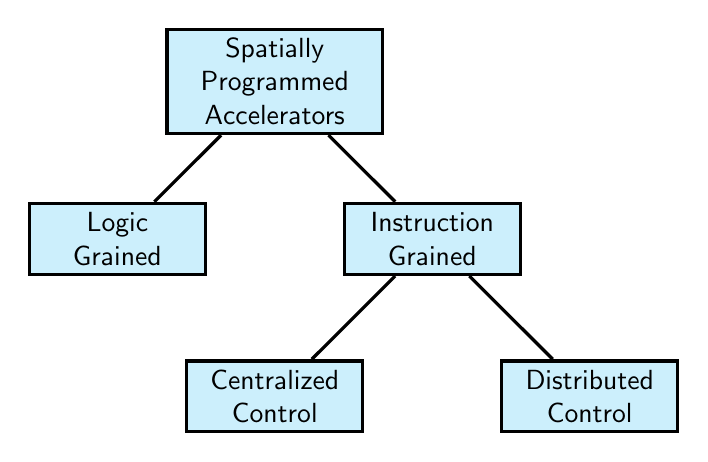
\begin{tikzpicture}[
      % For compatability with PGF CVS add the absolute option:
      absolute
      ]
      \begin{scope}[xshift=-7.5cm,yshift=-5cm,very thick,
        node distance=2cm,on grid,>=stealth',
        block/.style={rectangle,draw,font=\sffamily,fill=cyan!20,text width=2cm,text centered}]

        \node[block, text width=2.5cm] (spatial_acc) {Spatially Programmed Accelerators};
        \node[below=of spatial_acc]  (dummy1){};
        \node[block, left=of dummy1] (logic_grain) {Logic Grained};
        % \node[below=of logic_grain,yshift=35pt] (fpga) {FPGAs};
        \node[block, right=of dummy1] (inst) {Instruction Grained};
        \node[below=of inst] (dummy2){};
        \node[block, left=of dummy2] (cent_ctrl) {Centralized Control};
        \node[block, right=of dummy2] (dist_ctrl) {Distributed Control};
        \draw[-] (spatial_acc) -- (logic_grain);
        \draw[-] (spatial_acc) -- (inst);
        \draw[-] (inst) -- (cent_ctrl);
        \draw[-] (inst) -- (dist_ctrl);
      \end{scope}

    \end{tikzpicture}
  }
  \caption{Spatial Architectures classification \cite{parashar2014efficient}.} \label{fig:spatial_class}
\end{figure}

%This section will contain the relevant background. Consider the following items:
%\begin{itemize}
%\item Taxonomy of accelerators
%\item Non-Volatile Memories
%\item Memory wall
%\item Static Data-Dependency Analysis
%\item System Under Analysis
%\end{itemize}

\begin{figure*}[!ht]
\begin{minipage}{.7\textwidth}
\includegraphics[width=\textwidth,left]{images/framework_v2.pdf}
  \caption{\small \frameworkname~Framework.}{}
  \label{fig:framework}
\end{minipage}%
\begin{minipage}{.3\textwidth}
    \centering
\includegraphics[width=.4\textwidth]{images/architecture_v2.pdf}
\caption{\small The system under analysis.
    }
\label{fig:system}
\end{minipage}
\squeezeup
\squeezeup
\end{figure*}
\section{The \frameworkname~framework}
\label{sec:framework}
The \frameworkname~framework, illustrated in Figure~\ref{fig:framework} takes two inputs, the \textit{Configuration Parameters} and an \textit{Application} - described in Section~\ref{ssec:app}, and automatically generates a set of hardware architectures, behaviorally equivalent to the input application.
%Ana: the sentence below was a repetition - can skip.
%Additionally, the analysis of area, power and latency of these architectures is automatically produced.
The generated hardware architectures can be realized as RTL implementations, using the \textit{architectural templates} described in Section~\ref{sec:arch_template}.
The rest of this section provides an overview of the design and implementation of \frameworkname.

%\vspace{-1mm}
%\subsection{Model of Execution}
\label{ssec:system_under_analysis}
%\vspace{-1mm}
The system architecture we assume in this work has two levels of memory and a spatial processor (Figure~\ref{fig:system}). Level 1 memory (L1M)\footnotemark, the first memory level, and the smaller one in size, uses SRAM as it needs to be physically close to the processor for faster access. The second level - Level 2 memory (L2M)\footnotemark[\value{footnote}] - is larger in size and can be implemented using any memory technology (on-chip or off-chip), even with different access latency for read and write operations. Note that L2M can run at a different clock speed and different IO width than the processor and L1M.
\footnotetext{These memories are not to be seen as caches; thus, no cache policies are needed: we schedule data movements at design time. This is why we call them "levels" instead of "layers", and we abbreviate them with L1M and L2M instead of L1 and L2.}


We assume a model of execution following the three steps from Figure~\ref{fig:system}. Initially, all the required input data for the application are available in L2M. The input data is transferred to the processor, using L1M as intermediate storage (step 1), the data is processed and the results are temporarily stored in L1M (step 2), and, finally, the data from L1M is transferred back to L2M (step 3). The data transfers between L2M and L1M are handled by a Direct Memory Access (DMA) controller. Note that our model of execution performs the steps in a pipelined manner, hence only part of the data will be stored in L1M at any given time.

%\frameworkname~lets the user specify the parameters of the L2M through the \textit{Configuration Parameters}. The L2M parameters are used to model the data transfer between L2M and L1M (see \ref{ssec:layer2_model} and \ref{ssec:l2_read_model}). The L2M model is used to compute arrival time of input elements in the L1M. The arrival time of the element in the L1M is then used by the Modified Interval Partitioning (MIP) algorithm  - see \ref{ssec:modified_interval_partitioning}, to produce spatial architectures having bandwidth close to the bandwidth of the L2M. This effectively reduces the instantiation of unrequired resources in both the L1M and the spatial processor.
%The L1M is composed of multiple banks having different depths. The number and depths of the banks composing the L1M is determined by the MIP as described in \ref{ssec:arch_tradeoffs}.

%Taking advantage of the possibility to produce stacked chip having levels produced using different manufacturing technologies we are able to explore different memory implementations at the L2 of the memory architecture.

%\begin{figure}[tb]
%\centering
%\includegraphics[width=0.25\columnwidth]{images/architecture.pdf}
%\caption{\small The system under analysis. Composed by two levels of memory, the memory at layer two can use various technologies while the memory at layer one uses only SRAM technology.}
%\label{fig:system}
%\end{figure}

%\vspace{-1mm}
%\subsection{The L2 Memory Model}
\label{ssec:layer2_model}
%\vspace{-1mm}
Because L2M has higher access latency compared to the L1M and spatial processor, we model the L2M assuming its data is accessed in bursts.
%Figure~\ref{fig:l2model}  shows a representation of such access.
A read or write burst access to the L2M is controlled by a Direct Memory Access (DMA) controller, with the starting address and size of the burst given as input to the DMA. After an initial \textit{setup latency}, the accessed elements are transferred in sequence from the start address to the end address, from L1M to L2M in case of a write, and from L2M to L1M in case of a read.

\section{\frameworkname: Inputs}
This section details the two inputs of \frameworkname: the \textit{application} and the \textit{Configuration Parameters}.
%\vspace{-1mm}
%\subsection{Application}
\label{ssec:app}
%\vspace{-1mm}
The applications that can be used as input to \frameworkname~are completely defined at compile time, having control-flow instructions not dependent on input data. Such applications allow the static extraction of data dependency information performed by the \textit{Data Dependency Analysis} module (\ref{ssec:dda}). We currently support C/C++ applications. However, as the framework uses the LLVM Intermediate Representation~\cite{llvm}, it can be easily extended to support other languages as well.
%\begin{lstlisting}[language=C, caption={Example of input application, C implementation of a matrix vector multiplication.}, label={lst:matrixvec}]
%void matrix_vec_kernel(int *A,int *B, int *C){
%    int sum;
%    for(int i=0;i<DIM2;i++){
%        sum=0;
%        for(int j=0;j<DIM1;j++){
%            sum+=A[i*DIM1+j]*B[j];
%        }
%        C[i]=sum;
%    }
%}
%\end{lstlisting}

%\vspace{-1mm}
%\subsection{Configuration Parameters}
\label{ssec:conf_param}
%\vspace{-1mm}
The second input to the framework is a configuration file for the different building blocks to be used for hardware architecture realization. Through this file, the user can specify: different compute units (e.g. multipliers, adders), process technology to be used (e.g. 16nm, 28nm), the clock frequency of the processor and L1M, and the clock frequency L2M. Moreover, the user can specify the data-width used by the compute units, L1M and L2M.
Information to model the L2M burst accesses is also specified in this file: the setup latency for write/read accesses, the type of L2M to be used (e.g. MRAM, SRAM) and the size of the L2M. The different parameters in the configuration file are then used to access a database containing estimates (obtained by synthesis or from specs) of area usage, static and dynamic power, and latency of each of the building blocks. %Our L1M implementation uses multiple memory banks of different sizes (see \ref{ssec:arch_tradeoffs}). To estimate the resource usage of the different types of these memories we built a linear model, using synthesis data. We compared the ability of our linear model to predict area, latency and power consumption against the data generated using the synthesis tool and we found it to be accurate - less then 2\% error in the area and static energy model and less than 28\% error in the dynamic energy model.

%\begin{lstlisting}[language=json, caption={Example of input configuration file}, label={lst:conf_file}]
%{
%   "resource_database": {
%	"technology": 16,
%	"clock_frequency": 1000,
%	"bitwidth_adder": 128,
%	"bitwidth_multiplier": 64,
%	"bitwidth_register_file": 128,
%	"type_l2": "tt1v1v85c",
%	"technology_l2": 16,
%	"clock_l2": 800,
%	"bitwidth_l2": 32,
%	"depth_l2":2048,
%	"setup_write_latency_l2":2,
%	"setup_read_latency_l2":2
%   }
%}
%
%\end{lstlisting}

\section{\frameworkname: Analysis}
This section describes the parts of the framework involved in modeling the data transfers between L2M and L1M, \textit{Model L2 read} and \textit{Model L2 write} (\ref{ssec:l2_read_model}), the modules that perform data dependence analysis, \textit{Data Dependency Analysis} (\ref{ssec:dda}), and the scheduling of the application operations (\ref{ssec:modified_interval_partitioning}).
\vspace{-1mm}
\subsection{L2 Memory Read and Write Modeling}
\label{ssec:l2_read_model}
\vspace{-1mm}
The first operation performed by the framework is to compute the transfer time of the application's input data from L2M to L1M, implemented in the \textit{Model L2 read} block of Figure \ref{fig:framework}. Using static analysis, we obtain details regarding the data structures used in the application. For example, in a matrix vector multiplication kernel, the static analysis extracts information about three data structures: an input matrix and an input vector, containing the input elements of the computation, and an output vector containing the results. An address in L2M is given to each input element used by the application; different data structures are placed in consecutive memory addresses. The entire data transfer is modeled as a single burst-read operation from L2M. The information required to compute the arrival clock cycle of each input element to L1M is extracted from the \textit{Configuration Parameters}.
Using this information, the exact clock at which each input element arrives in L1M can be computed as seen in (1). The equation symbols are described in Table~\ref{table:equation}.

\begin{equation}
AClk_i = S_r + R_{L2M} * (Add_{L2Mi}+1) * \frac{B_{L1M}}{B_{L2M}} * \frac{Clk_{L1M}}{Clk_{L2M}}
\end{equation}

\begin{table}[]
\centering
%\footnotesize
\scriptsize
\begin{tabular}{|l|l|}
\hline
\textbf{Symbol} & \textbf{Definition}                                           \\ \hline
$AClk_i$           & Clock at which element i arrives to L1M                \\
$S_r$             & Setup Latency of a L2M burst read                          \\
$R_{L2M}$       & L2M read latency (per read), in L2M clock cycles   \\
$Add_{L2Mi}$     & Offset of element i in the burst access \\
$B_{L1M}$        & Data bitwidth of L1M                                       \\
$B_{L2M}$        & Data bitwidth of L2M                                       \\
$Clk_{L1M}$      & Clock Frequency of L1M                                     \\
$Clk_{L2M}$      & Clock Frequency of L2M                                     \\
$WBL_{L2M}$      & L2M write burst latency                                    \\
$S_w$             & Setup Latency of a L2M burst write                         \\
$W_{L2M}$       & L2M write latency (per write) in L2M clock cycles  \\
$O$                 & Total number of output elements                            \\ \hline
\end{tabular}
\caption{\small Definition of symbols used in the equations}
\label{table:equation}
\squeezeup
\squeezeup
\end{table}
The schedule produced by the Modified Interval Partitioning (MIP), discussed in \ref{ssec:modified_interval_partitioning}, uses the arrival clock cycle computed in this phase to determine when each input element will be available for computation in L1M. The latency of the MIP schedule includes therefore the L2M$\rightarrow$L1M transfer, and the computation; it does not take into account the L1M$\rightarrow$L2M transfer of the results (phase 3 in Figure~\ref{fig:system}).
The \textit{Model L2 write} block in Figure \ref{fig:framework} computes the latency of the L1M$\rightarrow$L2M transfer. The MIP computes the clock cycle at which computation ends (phase 2 in Figure~\ref{fig:system}) and the last data item is written in L1M. The L1M$\rightarrow$L2M transfer can start immediately after the last output is generated.
The latency of the L1M$\rightarrow$L2M transfer is calculated using (2),
\begin{equation}
    WBL_{L2M} = S_w + W_{L2M} * O * \frac{B_{L2M}}{B_{L1M}} * \frac{Clk_{L1M}}{Clk_{L2M}}
\end{equation}
where the symbols have been defined in Table~\ref{table:equation}.


\vspace{-1mm}
\subsection{Data Dependency Analysis}
\label{ssec:dda}
\vspace{-1mm}
The \textit{Data Dependency Analysis (DDA)} module operates in three stages. The first two stages are the extraction of the \textit{Data Dependency Graph} (DDG)\cite{isoda1983global} from the application and the schedule of the DDG using the As Soon As Possible (ASAP) and As Late As Possible (ALAP) methodologies. These two steps are core elements in the analysis of high level code for hardware design\cite{hwang1991formal}. Finally, the third step (see \ref{ssec:modified_interval_partitioning}) maps DDG instructions to hardware components - or PEs - using a modified \textit{Interval Partitioning} algorithm~\cite{greedyIntervalPartitioning}.
%This next paragraph might be replaced with a reference

%To extract the DDG from an application, we use LLVM  and custom transformations. We first convert the input application code to its LLVM Intermediate Representation. We then transform the code into static single assignment (SSA) form and perform full-loop unrolling on all of the application loops. After these transformations, there will be no control flow instructions in the application body, and each variable will be defined only once. It is now possible to follow the definition and use chain of the variables to produce a Data Dependency Graph like the one shown in Figure~\ref{fig:ddg}. The DDG represents each operation as a node - in Figure~\ref{fig:ddg} the input and output nodes represent respectively load and store instructions, while oval nodes represent computations - and each edge represents a dependency between operations.

We extract the DGG from the application using some LLVM optimizations and some custom code. We further process the obtained DDG, aiming to reduce the length of the path between the input nodes and the output nodes. This additional transformation is important because the length of these paths is equivalent to the number of sequential operations required to obtain the outputs, which in turn determines the latency of the application. Taking advantage of operation associativity (where possible) we can transform a long sequence of operations - like the one highlighted in Figure~\ref{fig:ddg} - into an equivalent shorter tree.
%\begin{figure}[ht]
%\begin{minipage}{.5\textwidth}
%\includegraphics[width=.9\textwidth,left]{images/supernode.pdf}
%  \caption{\small \frameworkname~Framework.}{}
%  \label{fig:framework}
%\end{minipage}%
%\begin{minipage}{.5\textwidth}
%    \centering
%\includegraphics[width=.9\textwidth]{images/supernode_optimized.pdf}
%\caption{\small The system under analysis.
%    %Composed by two levels of memory, the memory at layer two can use various technologies while the memory at layer one uses only SRAM technology.
%    }
%\label{fig:system}
%\end{minipage}
%\end{figure}

\begin{figure}[tb]
\centering
\includegraphics[width=.9\columnwidth,left]{images/supernode_2.pdf}
\caption{\small A Data Dependency Graph: inverse triangles represent input data, obtained from the \textit{load} instructions; ovals describe operations on data; the triangle at the bottom represents the result, derived from a \textit{store} instruction. Highlighted, a chain of associative operations before being optimized by the \textit{DDA} module (\ref{ssec:dda}).}
\label{fig:ddg}
\end{figure}

%This next paragraph might be replaced with a reference, we are interested mainly in the concept of mobility
Next, we apply the ASAP and ALAP scheduling methodologies\cite{hwang1991formal} to the generated DDG. These schedules will associate to each DDG node a clock cycle where the instruction is executed, and \textit{bound} the design space of possible architectures by determining the \textit{maximally parallel} architectures. We start by scheduling the input nodes of the DDG using the arrival clock time of their input data, computed as explained in Section~\ref{ssec:l2_read_model}, thus taking into account the L2M - L1M transfer time. Next, we determine the minimal latency required to obtain the outputs of the application with the ASAP schedule: starting from the DDG input leafs, each instruction node is scheduled as soon as its dependencies are resolved.
Once ASAP is completed, we can perform the ALAP scheduling: starting from the output leaf nodes, each node is scheduled as late as possible according to its dependencies. Once ALAP is completed, every node is annotated with an ASAP clock cycle and an ALAP one. The difference between these two clock cycles, called instruction \textit{mobility}, identifies an interval in which the instruction can be scheduled without changing the overall latency of the application.

The final stage of the \textit{Data Dependency Analysis} module will allocate the DDG nodes to PEs, leveraging the nodes mobility to minimize the number of PEs of the final hardware architecture.

\vspace{-2mm}
\subsection{PE allocation with Modified Interval Partitioning}
\label{ssec:modified_interval_partitioning}
\vspace{-1mm}
To generate a hardware architecture behaviorally equivalent to the input application and with the latency identified during the ASAP-ALAP scheduling, there are two main requirements: (1) each instruction needs to be computed within its ASAP-ALAP interval, and (2) instructions in the DDG which are executed by the same PE cannot be scheduled at the same time.
Our Modified Interval Partitioning (MIP) algorithm - based on the original greedy Interval Partitioning algorithm~\cite{greedyIntervalPartitioning} - is designed to generate, from a DDG, hardware architectures that meet both requirements. The original Interval Partitioning problem addresses the issue of assigning a number of jobs, with known starting and ending time, to the minimum amount of resources, ensuring that the jobs assigned to a resource do not overlap.


To use Interval Partitioning for our problem, we consider instructions as jobs and PEs as resources. There are, however, three main differences between our problem and the canonical Interval Partitioning.
First, the original algorithm considers any job can use any resource, while our architecture requires different PEs for different instructions. We therefore perform interval partitioning several times, once for each instruction type (e.g., four times for the graph in Figure \ref{fig:ddg}). This ensures a correct allocation of instructions to PEs performing the same operation.
Second, due to \textit{mobility}, instructions do not have a fixed starting time. MIP takes the mobility of an instruction into account by allowing a given instruction to start at any time within its allowed interval.
Third, our instructions are dependent on each other, which is not the case for the jobs in the original interval partitioning. To account for this extra constraint, we ensure that any given instruction (a) is only allocated after its dependencies are allocated, and (b) is scheduled to start after the ending time of its dependencies.
%Listing~\ref{lst:modified_interval_partitioning} presents MIP, in pseudo-code. %of our modified interval partitioning algorithm.

%\begin{lstlisting}[language=Python, caption={\small Modified Interval Partitioning (MIP) Algorithm}, label={lst:modified_interval_partitioning}, basicstyle=\tiny]
%# ASAP[i] and ALAP[i] contain the scheduled cycles for instruction i
%# SetPEs is the set of Processing Elements in the architecture
%SetPEs=[]
%sort instructions by ASAP[i]
%for each instruction i%
%	allocated = False
%	dep_deadline = maximum end-time of all instructions depending on i
%	schedule[i] = max(ASAP[i], dep_deadline)
%	for each PE in SetPEs
%		if instruction i matches PE
%			if ALAP[i] >=  next_free_slot[PE]
%				add instruction i to PE
%				schedule[i] = max(schedule[i], next_free_slot[PE])
%				next_free_slot[PE] = schedule[i] + latency(i)
%				allocated = True
%	if not allocated
%		create new PE with type(i)
%		add instruction i to PE
%		next_free_slot[PE] = schedule[i] + latency(i)
%		add PE to setPEs
%\end{lstlisting}

%We assume that ASAP and ALAP schedules have been previously performed, hence we can have two data structures that return the ASAP and ALAP schedules for a given instruction i - i.e. ASAP[i] and ALAP[i].
%Instructions is an ordered list of instructions initialized with the instructions of the input application.
%A Functional Unit is represented as a set containing the instructions that have been allocated to it, and FunctionalUnits is a set containing the Functional Units of the resulting architecture which is initialized as an empty set.
%The functions latency and dep take an instruction i as input and return respectively the latency of i and a list of instructions i depends on.
%The function type takes as input a Functional Unit or an Instruction and returns the type of operation performed.

%The MIP algorithm returns \verb|setPEs| and a \verb|schedule| for the current design: \verb|setPEs| is the list of processing elements that form the architecture, with each PE containing the instructions it has to execute, while \verb|schedule| contains the clock cycle at which each instruction is scheduled to be executed.

\vspace{-1mm}
\subsection{Most Parallel and Most Sequential Architectures}
\vspace{-1mm}
The result of the \textit{DDA} module is the \textbf{Most Parallel Architecture (MostPar)}. This architecture takes full advantage of the parallelism of the application and performs the computation with the minimum latency. However, MostPar uses the maximum number of PEs - in the worst case scenario equivalent to the number of instructions in the application - and it will hence have the largest area.
At the other end of the spectrum of architectures we can imagine the \textbf{Most Sequential Architecture (MostSeq)}, where no parallelism is used and the instruction are scheduled sequentially respecting their dependencies. This architecture will have the worst possible latency, but the minimal impact in area - using only one PE per operation type.
Probably none of these two architectures will be of direct interest for the user as they represent two extreme cases. Instead, the interesting architectures are the ones \textit{in between} \textbf{MostSeq} and \textbf{MostPar}, because they offer interesting trade-offs between power, latency and area. Section~\ref{ssec:dse} describes how these intermediate architectures can be generated using \textbf{MostPar} and \textbf{MostSeq}, respectively, as upper and lower bounds of the design space.

\section{\frameworkname: Design Space Exploration (DSE)}
%\vspace{-1mm}
%\subsection{Design Space Exploration}
\label{ssec:dse}
%\vspace{-1mm}
The \textit{Design Space Exploration} \frameworkname~module generates hardware architectures, behaviorally equivalent to the input application, which exhibit area, latency and power tradeoffs.
Our DSE is an iterative process which produces, at the end of each iteration, a different hardware architecture.
The iterative process starts its sweep from \textbf{MostPar}, and ends when \textbf{MostSeq} is generated.
%\begin{lstlisting}[language=Python, caption={\small Design Space Exploration},label={lst:dse},basicstyle=\tiny]
%currentArchitecture = MostPar
%found_MostSeq=False
%GeneratedArchitectures=[]
%while(!found_MostSeq)
%    type_count={}
%    found_MostSeq=True
%    for each PE in currentArchitecture
%        type_count[type(PE)]+=1
%            if type_count[type(PE)] > 1
%                found_MostSeq=False
%                break
%    if found_MostSeq
%       break
%    for each instuction i in DDG
%        if type(i) == 'store'
%            ALAP[i] = ALAP[i]+1
%    ALAP=performALAPschedule(instructions,dependencies)
%    SetPEs=MIP(instructions,ASAP,ALAP)
%    GeneratedArchitectures+=[SetPEs]
%    currentArchitecture=SetPEs
%\end{lstlisting}
An iteration consists of three steps. First, the instructions corresponding to output leaf nodes in the DDG are selected. The ALAP schedule of these iterations is increased by 1, and the ALAP scheduling of the rest of the nodes in the DDG is updated accordingly. Consequently, the mobility of each instruction node is increased by one. Finally, the MIP is ran again, using the new ALAP schedule. Due to the increased mobility of each instruction, the generated architecture is likely to use less PEs.
The process stops as soon as it generates \textbf{MostSeq}, which can be recognized because it contains only one PE per operation type.

Users can tune the DSE process, trading speed for completeness: by increasing the ALAP "slack" beyond 1, the exploration speeds-up, but less architectures are generated.

%This has been merged with the L2 Memory Read section
%\vspace{-1mm}
%\subsection{L2 Memory Write}
%\vspace{-1mm}
%The schedule produced by MIP includes the L2M-L1M transfer, and the computation; it does not include the L1M-L2M transfer. However, due to MIP, we do know the clock cycle at which computation ends (phase 2 in Figure~\ref{fig:system}) and the last data item is written in L1M. The L1M-L2M transfer can start immediately after the last output is generated.
%The latency of the L1M-L2M transfer is calculated using (2),
%\begin{equation}
%    WBL_{L2M} = S_w + W_{L2M} * O * \frac{B_{L2M}}{B_{L1M}} * \frac{Clk_{L1M}}{Clk_{L2M}}
%\end{equation}
%where the symbols have been defined in Table~\ref{table:equation}


%\vspace{-1mm}
%\subsection{Architecture Tradeoffs}
%\label{ssec:arch_tradeoffs}
%\vspace{-1mm}
%In section~\ref{
%For a given input application and a given configuration, \frameworkname~outputs a set of hardware architectures - composed of spatial processor and L1M - with different area and latency trade-offs. Figure~\ref{fig:tradeoffs} shows three of the architectures generated during the DSE. Each box represents a PE. The different load and store PEs are implemented as separate L1M banks. As an example, the architecture in Figure \ref{fig:inter_arch} has 1 L1M bank to store the input data and 5 banks to store the results. This architecture can therefore receive 1 input element per clock cycle from the L2M, and store up to 5 results per clock in the L1M store banks. The remaining PEs are obtained from computing instructions. We allow the architectures to have cycles because the circuit is synchronous, and every instruction has been carefully scheduled. A self-loop in a PE indicates data reuse (see Section~\ref{sec:arch_template} for implementation details).
%\begin{figure}[ht]
%\centering
%\begin{subfigure}{.4\columnwidth}
%  \centering
%  \includegraphics[width=\textwidth]{images/Architecture_latency_146_schematic.png}
%  \caption{}
%  \label{fig:max_par_arch}
%\end{subfigure}%
%\begin{subfigure}{.3\columnwidth}
%  \centering
%  \includegraphics[width=\textwidth]{images/Architecture_latency_166_schematic.png}
%  \caption{}
%  \label{fig:inter_arch}
%\end{subfigure}
%\begin{subfigure}{.2\columnwidth}
%  \centering
%  \includegraphics[width=0.5\textwidth]{images/Architecture_latency_188_schematic.png}
%  \caption{}
%  \label{fig:most_seq_arch}
%\end{subfigure}
%    \caption{\small Example of architectures generated from a matrix vector multiply application of size 5x5. The MostPar (a), an intermediate architecture (b) and the MostSeq (c).}
%\label{fig:tradeoffs}
%\end{figure}


%\subsection{Multi-Configuration Design Space Exploration}
%\label{ssec:multiconf_dse}
%\frameworkname~can also perform design space exploration on the configuration parameters (Section~\ref{ssec:conf_param}), generating one configuration file for each combination of configuration parameters and aggregating the architectural trade-offs. This allows, as an example, to estimate the effect that different clock frequencies or different memory technology have on the area,latency and energy trade-offs. The use cases discussed in \ref{ssec:case_study2} and \ref{ssec:case_study3} are examples of multi-configuration DSEs.
%\begin{figure}
%
%\begin{minipage}{.5\linewidth}
%\centering
%\subfloat[]{\label{main:a}\includegraphics[scale=.2]{images/Architecture_latency_188_schematic.png}}
%\end{minipage}%
%\begin{minipage}{.5\linewidth}
%\centering
%\subfloat[]{\label{main:b}\includegraphics[scale=.2]{images/Architecture_latency_166_schematic.png}}
%\end{minipage}\par\medskip
%\centering
%\subfloat[]{\label{main:c}\includegraphics[scale=.10]{images/Architecture_latency_146_schematic.png}}
%
%\caption{my fig}
%\label{fig:main}
%\end{figure}

\vspace{-2mm}
\section{Architectural Template}
\label{sec:arch_template}
To implement the architectures generated by \frameworkname in hardware, we propose a PE template, shown in Figure~\ref{fig:FU_templ}. Each PE has an Instruction Memory (IM) where the operations to be performed at each clock cycle are stored. Each instruction is labeled with the clock cycle in which it should be scheduled. An internal clock counter is compared to the label to decide when to issue the instruction. The internal Register Files (RFs) are used to store input data that needs to be processed in the future, as well as output data that needs to be reused. The \textit{X-bar} in the diagram represent configurable crossbars, which can send data from any input port to any output port. OP is the hardware unit that performs an arithmetic (or logical) operation - e.g. add or multiply.
This PE template allows modular implementation of the spatial processor architecture - given that the instructions to execute are stored in the local IM. The inputs to a PE can either be generated by other PEs or the output generated by the same PE in the previous clock cycle. In addition, the inputs to the PE can be used as operands for immediate computation or stored in the RFs for future use. %We have implemented the template PE in RTL that can be configured to build all types of PEs found in the architectures generated by \frameworkname.

\begin{figure}[tb]
\centering
\includegraphics[width=.5\columnwidth]{images/functional_unit.pdf}
    \caption{\small Functional Unit template. PE1-PE4 represent "parent" PEs that generate input data. IM is an internal Instruction Memory,where the PE stores the operations to be performed. RFs are internal Register Files, which store reuse data and inputs to be used in the future. OP is the hardware unit actually performing the PE operation.}
\label{fig:FU_templ}
\squeezeup
\squeezeup
\end{figure}

\begin{figure*}[ht]
\centering
\begin{subfigure}{.33\textwidth}
  \centering
  \includegraphics[width=\textwidth]{graphs/energy_plot_single_sram.pdf}
  \caption{5x5 MM}
  \label{fig:single_sram}
\end{subfigure}%
\begin{subfigure}{.33\textwidth}
  \centering
  \includegraphics[width=\textwidth]{graphs/EnergyParetoMatrixVec10.pdf}
  \caption{MV 10x10}
  \label{fig:sram_vs_mram_pareto_vec}
\end{subfigure}
\begin{subfigure}{.33\textwidth}
  \centering
  \includegraphics[width=\textwidth]{graphs/EnergyParetoMatrixMul10.pdf}
  \caption{MM 10x10}
  \label{fig:sram_vs_mram_pareto_mul}
\end{subfigure}
    \caption{\small Each point represents one \frameworkname~spatial processor. Different shapes (in \ref{fig:sram_vs_mram_pareto_vec} and~\ref{fig:sram_vs_mram_pareto_mul}) identify different input configurations. \ref{fig:single_sram} shows the architecture's Energy over Latency in clock cycles generated from a single configuration of a matrix vector multiplication of size $5\times5$. Note that (a) presents all designs, while (b) and (c) only include the Pareto-optimal designs.}
\label{fig:case_studies_1}
\end{figure*}
\section{Case Studies}
\label{sec:case_studies}
In this section, we demonstrate the capabilities of \frameworkname~using three case studies. To do so, we analyze the architectures generated by \frameworkname~and the energy consumption and latency of each design.
We selected two representative applications: matrix-vector (MV) and matrix-matrix (MM) multiplication with matrix sizes $5\times5$, $10\times10$, and $15\times15$. We used the TSMC 28nm target technology library for generating the database containing the area usage and energy consumption of the different building blocks, as required by our framework.
We generated multiple input \textit{Configuration Parameters} - Section~\ref{ssec:conf_param} - to let \frameworkname~select the correct building blocks data from the database, and compute the latency, area usage, and energy consumption of the architectures. Each generated architecture has a known latency imposed in each iteration of the DSE(Section~\ref{ssec:dse}), which we use to compute its static energy consumption. Moreover, after applying the Modified Interval Partitioning algorithm (see Section~\ref{ssec:modified_interval_partitioning}), the instructions performed by each PE are known and this information is used to compute the dynamic energy consumption of an architecture.

In the first case study - Section~\ref{ssec:exp_single} - we illustrate how DSE works for 5x5 MV and a single configuration. The second case study compares the use of MRAM - modeled according to~\cite{8310393} - and SRAM for L2M (both in 28nm) for the two applications. The last case study compares \frameworkname~architectures for the different MV sizes.

\vspace{-1mm}
\subsection{Single configuration DSE}
\label{ssec:exp_single}
\vspace{-1mm}
The goal of this case-study is to illustrate the ability of \frameworkname~to generate, given a single configuration, architectures with different energy consumption. The configuration uses SRAM in both levels. L2M is clocked at 350MHz, while L1M and the spatial processor are clocked at 1GHz. Figure 7a shows the energy consumption of 30 different \frameworkname~designs, with different latency. We make two observations: (1) the latency and power consumption of each design range between the min and max latency, as given by the \textbf{MostPar} and \textbf{MostSeq} architectures, and (2) as expected, faster designs result in higher energy consumption, due to their larger numbers of PEs.

%The \textbf{MostPar} - starting point of our DSE - is the fastest architecture completing the computation in 412 clock cycles of the spatial processor and it consumes $11.1^3$ mW-ns. The \textbf{MostSeq} - ending point of the DSE - is the slowest, completing in 436 clock cycles and consuming $6^3$ mW-ns. Between these two extreme design points, the DSE generates intermediate architectures with various energy-latency tradeoffs.

\vspace{-1mm}
\subsection{MRAM vs SRAM Level 2 Memory}
\label{ssec:case_study2}
\vspace{-1mm}

In this case study we compare the power efficiency of two alternative technologies to implement L2: MRAM and SRAM.
The comparison is performed using both applications - MV and MM - with $10\times10$ matrices (see Fig~\ref{fig:sram_vs_mram_pareto_vec} and~\ref{fig:sram_vs_mram_pareto_vec}, respectively). In both graphs, each point is relative to a hardware architecture generated by \frameworkname; moreover shapes identify different input configurations. Specifically, we compare a total of 18 configurations: 2 L2M technologies, MRAM and SRAM, clocked at 350MHz, and 9 different clock frequencies (400MHz - 1GHz, in steps of 200) for the processor and L1M ensemble.

In both figures we can identify two clusters: HE-LL (high-energy, low-latency) and LE-HL (low-energy, high-latency). Each cluster belongs to one memory technology: HE-LL contains of all SRAM designs, while LE-HL containts all MRAM designs.
For the MV application (Fig~\ref{fig:sram_vs_mram_pareto_vec}) the fastest architecture - using SRAM memory - has a latency of 1375ns and consumes over $1^5$mW-ns. The most energy efficient SRAM architecture has instead a latency of 1525ns and consumes under $0.3^5$mW-ns, thus being 3x more energy efficient than the fastest with a 10\% increase in latency. The most energy efficient architecture using MRAM technology has instead a latency of 2210ns and consumes $0,24^5$mw-ns, hence having 45\% higher latency than the best SRAM counterpart, with 25\% lower power consumption. The matrix multiplication, Figure~\ref{fig:sram_vs_mram_pareto_mul}, performs 10 times more operation than the matrix vector multiplication, hence there is a clear overall increase in latency - about 30\% - and energy consumption - about 4 times -  in comparison to the previous application. In this case the architecture using SRAM consuming the least amount of energy is has 2\% higher latency compared to the fastest one, but consumes 50\% less energy. However, the introduction of MRAM technology in the L2M is not as beneficial as it was for the matrix vector application. The MRAM architecture consuming the least amount of energy has a 3\% slowdown compared to the most energy efficient SRAM, while attaining only a 2.2\% improvement in energy consumption.

\begin{table*}[!ht]
  \resizebox{\textwidth}{!}{%
\begin{tabular}{llllll}
Framework & Type (see \ref{sec:bg})    & Application Optimized & Memory Co-Design & Architectural DSE & High Level Language \\
\frameworkname         & Distributed Control       & Yes                   & Yes              & Yes               & Yes, C              \\
\cite{parashar2014efficient}               & Distributed Control       & No                    & No               & No                & No                  \\
\cite{prabhakar2017plasticine}               & Centralized Control       & No                    & No               & No                & Yes, DHDL           \\
\cite{streamproc2019}               & Distributed Control       & No                    & No               & No                & No           \\
\cite{budiu2004spatial}               & Design-Time Programmable & Yes                   & No               & No                & Yes, C \\
 \cite{cerqueira2020catena}              & Distributed Control  & Yes                   & No               & Yes                & No
\end{tabular}
}
\caption{Comparison with related work.}
\label{tab:rw}
\end{table*}

\subsection{Different Matrix Dimensions}
\label{ssec:case_study3}
In this case study we compare three different matrix sizes for MV - $5\times5$, $10\times10$ and $15\times15$, using the same configurations used in~\ref{ssec:case_study2}, to evaluate how the energy consumption of an L2M MRAM scale with respect to an L2M SRAM. Figure~\ref{fig:sram_vs_mram_pareto_vec_sizes} shows the Pareto-optimal architectures generated from each input application. The increase in the matrix size is reflected by an increase in latencyi: all MV-$5\times5$ application-specific processors have latency below 1000ns, MV-$10\times10$ processors latency range between 1250ns and 2500ns, and the MV-$15\times15$ processors have latency beyond 2500ns.
However, the increased number of operations results instead in wider trade-offs possibilities. Thus, the normalized latency gap between the most energy efficient SRAM and MRAM, decreases with the matrix size, from 82\% for the $5\times5$, to 42\% for the 10x10 and even 32\% for the $15\times15$. The reduction in energy consumption between the same pair of results is instead 20\% for the $5\times5$ and $10\times10$, while for the $15\times15$ drops to 16\%. Therefore, as the size of the matrix grows, the benefits in energy consumption reduces when using MRAM technology in the L2M. This is a behaviour caused by the increased number of write operations that have high energy impact when the MRAM technology is used.



\begin{figure}[!h]
\centering
\includegraphics[width=0.33\textwidth]{graphs/EnergyParetoPlotMultipleSizeMAtrixVec.pdf}
    \caption{\small Energy Pareto optimal architectures generated by \frameworkname ~for different sizes of Matrix Vector multiplication 5x5 - with latency ranging from 0 to 1000,10x10 - having latency between 1000ns and 2500ns , and 15x15- with latency above 2500ns. Each point corresponds to an architecture generated by the framework.}
\label{fig:sram_vs_mram_pareto_vec_sizes}
\end{figure}


\section{Related Work}

%Prior art on design-space exploration of custom or domain-specific processors~\cite{Jordans2014,EusseSAMOS2014,Jozwiak2013} aims to find the optimal processor architecture in terms of area usage, power consumption and execution cycles. Processors with Single Instruction Multiple Data (SIMD) or Single Instruction Multiple Threads (SIMT) are typically used for data-flow or streaming applications. SIMD and SIMT architectures are not scalable due to a single Instruction Memory. Spatial architectures~\cite{7284058,8686088} helps to distribute the Instruction Memory and achieve a higher clock speed. State-of-the-art Spatial archiectures are designed for maximum flexibility and provide connections from any ALU or PE to any other using an interconnect. Prior art on using non-volatile memories as a replacement L2 memory perform co-simulation of the processor and the memory system and optimizes the cache replacement policies~\cite{4798259,7092595,6271803,7360193,200116,Patel2016ReducingSL,Komalan:2014,Mittal13f}.

%For the energy model~\cite{Yannan2019}

%Papers to cite for CDFG generation and Application Specific High LSynthesis~\cite{Coussy:2008:HSA:1457713,Kato2008}



Previous work on designing spatial processor focuses on the hardware architecture of the processor, while the optimization of the memory system is only partially taken into account.
In \cite{parashar2014efficient} a spatial processor with distributed control across PE using triggered instructions is presented. Their architecture is built around the guarded-action programming paradigm, where guards - boolean expressions specifying if an action is legal - are evaluated by a scheduler and trigger computations. Support for high level languages is missing, so this spatial processor needs to be programmed in a low level guarded-action language and the computation needs to be manually mapped on the PEs. Their memory system consist of two levels of memories (L1 and L2) and distributed scratch-pad memories located within the PEs. The design is not tailored for a specific set of applications and they do not perform analysis on the interactions between the memory and processing systems, leaving the modeling of the memory system as future work.

Plasticine, a spatial processor optimized for the acceleration of parallel patterns is presented in \cite{prabhakar2017plasticine}. Their memory system is composed of Pattern Memory Units (PMUs) which are connected through a network to Pattern Compute Units (PCUs). Although it allows some degree of configuration, Plasticine is not meant to be optimized around specific applications. The input application needs to be written in a language exposing its parallel patterns - Delite Hardware Definition Language (DHDL) - and then it is mapped on the Plasticine architecture. Hence, the number of memory units (PMUs) and processing units (PCUs), and their interconnections are not optimized around specific applications.

In \cite{budiu2004spatial}, a framework to generate Application Specific Hardware (ASH) from a C application is presented. The final architecture it produces is asynchronous, and operation dependencies are handled using a token-based mechanism which is implemented in hardware. The memory system of the architecture consists of a monolithic memory. To handle concurrent memory requests the design uses a hierarchy of busses and arbiters, which creates a bottleneck. This means that their memory system is overwhelmed because it is not tailored for the PEs it uses.

Spatially distributed PEs with a dedicated configuration register allow to configure the PEs to one of the operating modes \cite{streamproc2019} at compile time. Few PEs are connected back-to-back, forming systolic arrays which are then interconnected using an on-chip interconnect. Thus, the processor architecture is quite general-purpose, i.e, the interconnect allows a PE array to be connected to any another PE array. However, there is no automated design flow to efficiently map algorithms to the processor architecture.

An interesting approach is Catena\cite{cerqueira2020catena}, an ultra-low-power spatial processor with a distributed architecture, where multiple techniques - \textit{clock gating}, \textit{power gating} and \textit{voltage boosting} - are applied in a fine-grained way to optimize energy efficiency. These techniques can be used to explore the power/latency tradeoff of specific applications. However, the impact of the memory system on the performance of the design is not modeled and the memory system is not co-designed with the spatial processor, potentially resulting in an inefficient utilization of the hardware resources; moreover, Catena lacks high-level language support.

In summary, a comparison of \frameworkname~against existing work is presented in Table \ref{tab:rw}.

\begin{table}[!ht]
 \resizebox{0.5\textwidth}{!}{%
\footnotesize
    \begin{tabular}{|l|l|l|l|l|l|}
      \hline
  Framework & Type    & Application & Memory & Architectural& High Level \\
           & (see \ref{sec:bg})    & Optimized & Co-Design &DSE & Language \\ \hline
\frameworkname         & Dist. Control       & Yes                   & Yes              & Yes               & Yes, C              \\ \hline
%            & Control       &                    &               &                &              \\ \hline
\cite{parashar2014efficient}               & Dist. Control       & No                    & No               & No                & No                  \\ \hline
%            & Control       &                    &                &                 &                   \\ \hline
\cite{prabhakar2017plasticine}               & Dist. Control       & No                    & No               & No                & Yes, DHDL         \\ \hline
            %&        &                     &                &                 & DHDL           \\ \hline
\cite{streamproc2019}               & Dist. Control       & No                    & No               & No                & No           \\ \hline
%            & Control       &                     &                &                 &            \\ \hline
\cite{budiu2004spatial}               & Logic & Yes                   & No               & No                & Yes, C \\
            & Grained &                    &                &                 &  \\ \hline
 \cite{cerqueira2020catena}              & Dist. Control  & Yes                   & No               & Yes                & No \\ \hline
%            & Control  &                    &                &                 &  \\ \hline
\end{tabular}
}
\caption{Comparison with related work.}
\label{tab:rw}
\end{table}

\section{Conclusion and Future Work}
In this work, we presented \frameworkname, a novel framework for co-designing memory-aware custom processors.
%with a two-level memory system. .
%Our framework enables the automatic design of a broad range of application-specific processors, using a two-level memory system.
The framework enables design-space exploration of spatial processor architectures including the memory system. We have empirically demonstrated that different spatial processor architectures can be quickly implemented using our novel PE hardware template. Lastly, we have shown the capabilities of the framework using a case study, which illustrate the sanity of our DSE approach and its ability to facilitate a comparison between the use of MRAM and SRAM technologies.
For example, we were able to conclude that, for a matrix vector multiplication 10x10, the most energy efficient architecture generated with \frameworkname~with MRAM L2M has 45\% higher latency than the best SRAM counterpart, with 25\% decrease in power consumption.

Our future work focuses on the use \frameworkname~to analyze multiple applications. In addition, we plan to enhance our framework adding the capability of automatically \textit{merging} multiple spatial processor architectures, to generate a single \textit{multi-application spatial processor}.

\section{Method}
\label{ch:method}
This chapter presents our method for constructing efficient multi-mode architectures. We start by considering possible efficiency metrics and their applicability in our case to answer RQ1. Next, we present the actual merging method, which combines two application-specific architectures, thus answering RQ2. Finally, we extend this method with a DSE, to find pairings within the sets of input architectures that result in efficient merged architectures, answering RQ3.

\section{Efficiency metrics}
The first step in our research is to establish which metrics to consider for efficiency. Doing so helps guide the creation of our method towards a shared goal, helping us decide the input and steps our method should take in order to best optimise these metrics.

We base our discussion on latency, area usage, and energy consumption, as these metrics are the most common in the HLS and DSE literature seen so far. The latency of an architecture represents the time needed to execute the program it implements, measured in clock cycles. Area usage refers to the amount of physical area required to implement the architecture on a chip. Lastly, the energy consumption is the amount of energy required to execute the application, and is divided into the passive energy, determined by passive leakage of electrical energy in hardware, and the dynamic energy, required to activate the components.

Out of these, area is the most important metric to us, as we are specifically aiming to design a merging method that exploits resource sharing. Because area is determined by component count and size, and the goal of resource sharing is to avoid unnecessary resource duplication, minimising the area of the merged architecture implies maximising resource re-use. Thus, our method aims to optimise the area of the merged architecture.

In contrast, the latency of the input applications in the output architecture is directly related to their latency in the original architectures. By selecting architectures with higher latencies, we can use less parallel and thus lower area architectures in our merge. To explore the different combinations of latency and area, we rely on the latency of the original architecture, and make use of the DSE process to select the pairs of architectures to merge.

Finally, energy is made up of two components, the static and dynamic energy. The dynamic energy of an application is determined mostly by the amount of operations in the application, and is thus largely constant regardless of architecture. On the other hand, the static energy is determined by the passive leakage of the hardware, and only depends on the area and latency. Because a merged architecture is larger than its inputs, running a program on a merged architecture incurs an energy overhead compared to running it on its original architecture. Thus, the energy consumption of the architecture is highly dependent on the values of the latency and area.

In conclusion, when merging input architectures, we prioritise minimising the area of the merged architecture, while preserving the latency of the input architectures, and minimising energy consumption.

\section{Merging method for architectures}
\label{method:method}
Our goal is to devise a method to merge two application-specific architectures as output by the \microgenie framework. The resulting architecture must be able to run each application individually, and minimise area and static energy while preserving the latency and dynamic energy of the original input architectures. We note that it is not necessary for applications to be able to run concurrently, as our goal is to be able to run \textit{either} application on the same hardware, rather than \textit{both} at the same time. We focus on creating the necessary \textit{hardware}, relying on a separate step to create the necessary hardware instructions to run the input applications on the merged hardware.

To meet these requirements, our method that merges two architectures, represented as graphs of FUs, has three major steps:
\begin{enumerate}
\item Isolate the maximum common subgraph \textit{mcs} of the input graphs.
\item Mapping the `leftover' nodes where possible.
\item Completing the graph with the remaining `leftovers'.
\end{enumerate}
We further present the motivation and procedure for each of these steps.

\subsection{Isolating the \textit{mcs}}
We begin the merge by isolating the \textit{mcs} of the input graphs to use as the `core' of our merged architecture. By definition, this is a subgraph that exists within both input graphs that is also maximum in its size compared to other common subgraphs. Thus, the \textit{mcs} represents the largest part of the input architectures that we can directly reuse in our result without introducing any additional hardware or overhead, as it is used in both original architectures. We note that multiple \textit{mcs} of equal size may exist for any pair of architectures, any one of these are valid for our method.

We solve the \textit{mcs} by transforming it to the maximum clique problem on the compatibility graph of the input graphs (as outlined in Section~\ref{bg:mcs}). We impose an additional restriction to the \textit{mcs} found in this manner: two FUs can only map onto each other if they perform the same operation in hardware. Because we rely on a separate step to implement the input applications on the merged hardware, we do not consider the instruction memory in the FUs for this restriction.

\subsection{Mapping leftovers}
After isolating the \textit{mcs}, we are left with two sets of `leftover' nodes. Our next step is to map together---that is, map on shared resources---any nodes of the same type between the two leftover sets. Pairing two nodes from the two different sets, and mapping each pair on a new shared resource creates \textit{one} new node in our merged graph, with all of the connections of both original nodes.

Matching these leftovers results in new nodes with edges that should only be active when one of the two applications is running, meaning that we must be able to ignore certain hardware connections at runtime. This is possible by adding switching hardware where these edges meet, allowing the hardware to select which of multiple inputs to connect to an output. In the FUs used in our framework, this functionality is provided by the crossbar.

Compared to the previous step, mapping FUs in this way creates additional hardware overhead, in the form of hardware connections that are used only in one of the two applications. These added connections increase the amount of control logic required in both the memory and hardware of the FU. When an FU has more connections, instructions require more bits to address the different connections to select the inputs, increasing the area of the instruction memory. More hardware is also needed in the crossbar of the FU itself, contributing to the overall area increase. To minimise the cost of this overhead, we prioritise mapping together FUs with overlapping edges leading to the same node.

Following this, we also note that, due to the way the partitioning algorithm used for allocation in \microgenie, the amount of components for a certain operation in an architecture is always equal to the maximum amount of operations of that kind that run in parallel at any point in the application. Consequently, the merged architecture should never need more of one kind of component than any of the original architectures. With maximum sharing, this means that the amount of components of a certain type in the merged architecture is exactly equal to the maximum amount of components of that type found in any of the two input architectures. Thus, we continue mapping the leftovers until we run out of compatible FUs implementing the same operation.

\subsection{Completing the graph}
As a final step, we \textit{add} all remaining leftovers---i.e., the FUs not mapped in the previous step---along with all their connections. Any nodes added at this point are guaranteed to belong to only one architecture. This leaves us with a supergraph containing both of the input graphs as non-induced subgraphs. This supergraph is capable of running both input programs by mapping the instruction memories from the input units to the corresponding units in the output architecture.

\section{Design-space exploration for efficiency}
\label{method:dse}
Our method so far allows us to merge any two architectures together. In order to explore the merge of the two input applications, one question remains: how we can select \textit{the right} pairs of architectures for the input applications, such that we can create efficient merged architectures? To address this problem, we perform a design-space exploration (DSE), wherein the space represents all possible pairings, while the selection of efficient ones is made using the proposed efficiency metrics. The full merging flow is shown in Figure~\ref{fig:full_flow}.

\begin{figure}[!htb]
    \centering
    \includegraphics[width=\textwidth]{graphs/full_flow.pdf}
    \caption{A view of our full merging flow. We use \microgenie to generate sets of architectures from the program descriptions. After merging these sets, we use a DSE process to find the merged architectures that are efficient.}
    \label{fig:full_flow}
\end{figure}

For DSE, we first define the design space as the complete set of possible architectures for the input applications, i.e., the Cartesian product of the sets of architectures for each input application. Doing so gives us access to pairs of architectures with different parameters for all of our efficiency metrics (area, latency, and energy consumption), ensuring the completeness of our design space.

Next, we analyse each merged architecture using our efficiency metrics. Because each resulting architecture is multi-mode, it has separate latency and energy metrics for each individual mode, because both of these metrics depend on the execution. By construction (as designed in Section~\ref{method:method}), the latency and dynamic energy of each mode are the same as in the original architecture, whereas the static energy \textit{changes}, because it depends on the area of the merged architecture.

Finally, in our exploration, we find the Pareto set of the merged architectures. To do this, we assume a scenario in which all modes run equally often, i.e., for every execution of application 1 there is also an execution of application 2. Under this scenario, we can approximate the latency and energy of the merged architecture as the sum of the latency and energy of both modes. We note that with this method, different exploration strategies can be used by changing the way the metrics are estimated according to the scenario.

Using this DSE approach, in which we explore merges of \textit{all} the individual architectures implementing \textit{each} of the two given applications, and \textit{select only the efficient ones}, we generalise from a method of merging two architectures to a method for merging two applications.

\section{Implementation}
\label{method:implementation}
This section presents the pseudocode and implementation details of the methods formulated in this chapter, accompanied by a running example that demonstrates the architecture merging method in practice, step by step. The input architectures for this example are shown in Figure~\ref{fig:running_example}.

\begin{figure}[!htb]
  \begin{subfigure}{\textwidth}
    \centering
    \includegraphics[scale=0.5]{graphs/running_example1.png}
    \caption{Architecture 1}
    \label{fig:running_example:a}
  \end{subfigure}\\
  \begin{subfigure}{\textwidth}
    \centering
    \includegraphics[scale=0.5]{graphs/running_example2.png}
    \caption{Architecture 2}
    \label{fig:running_example:b}
  \end{subfigure}
\caption{The input architectures of our running example. Architecture 1 has an extra \texttt{add\_1} node inserted compared to architecture 2.}
\label{fig:running_example}
\end{figure}

We calculate the \textit{mcs} on the input graphs with any self-edges removed. Since self-edges in the \microgenie output represent reads or writes from the component's own memory, these loops are irrelevant to the overall topology. However, the existence of loops in the graph would automatically mean that nodes containing them are non-isomorphic to nodes without them, and therefore cannot be matched as part of the \textit{mcs} algorithm. By removing such edges, we correctly maximise the coverage of the \textit{mcs}.

We find the \textit{mcs} by computing the maximum clique~\cite{konc2007improved}. on the compatibility graph between our two input graphs. We construct the edges of the compatibility graph by iterating over each pair of mappings in the compatibility graph, skipping any that map nodes of different types together. We add an edge between two mappings if they are \textit{compatible} (as defined in Section~\ref{bg:cg}). This construction is illustrated in Figure~\ref{fig:cgconstruction}. Each node in the maximum clique represents a pair of nodes, one from each input graph, which we map to each other to create the \textit{mcs}. Figure~\ref{fig:runningmcs} illustrates the \textit{mcs} for our running example.

\begin{figure}[!htb]
\begin{lstlisting}[title={Compatibility graph construction}, keywords={for, in, where, if, and}]
for vertex v1 in graph1:
    for vertex u1 in graph1, where v1 != u1:
        for vertex v2 in graph2, where v1.type == v2.type:
            for vertex u2 in graph2, where u1 != u2 and u1.type == u2.type:
                if edge_exists(v1, u1) == edge_exists(v2, u2):
                    add_edge(<v1,v2>, <u1,u2>)
\end{lstlisting}
    \caption{Pseudocode of the compatibility graph construction from two input graphs, where \texttt{v1} and \texttt{u1} are vertices in graph 1 and \texttt{v2} and \texttt{u2} are vertices in graph 2.}
    \label{fig:cgconstruction}
\end{figure}

\begin{figure}[!htb]
    \centering
    \includegraphics[scale=0.5]{graphs/running_example1+running_example2_mcs.png}
    \caption{The disconnected \textit{mcs} of the running example.}
    \label{fig:runningmcs}
\end{figure}

With the \textit{mcs} ready, we create the two leftover sets of nodes from each architecture by iterating over each node, adding any that are not part of the \textit{mcs} to the leftovers. We map the leftover nodes by type, and minimise the creation of new edges by selecting nodes with matching edges in the process. We do so by counting the amount of overlapping edges for each pair, and selecting the pairs with the most overlap. Edges are considered overlapping if the nodes connected to them map to each other, ignoring nodes that are not yet mapped. Figure~\ref{fig:mapping} shows the pseudocode for the matching algorithm, and Figure~\ref{fig:runningextended} illustrates the graph resulting from applying this to our running example, with the \textit{mcs} highlighted in red and the extended leftovers in blue.

\begin{figure}[!htb]
\begin{lstlisting}[title={Mapping leftovers}, keywords={for, in, where, if, while, and}]
while new pair possible:
    for vertex v in leftovers_in_graph1:
        for vertex u in leftovers_in_graph2, where v.type == u.type:
            overlap = 0

            for vertex a in adjacent_vertices(v):
                if equivalent_vertex_in_graph_2(a) in adjacent_vertices(u):
                    overlap += 1

            if overlap > max_overlap:
                best_pair = <v,u>
                max_overlap = overlap

    add_vertex_from_mapping(best_pair)
\end{lstlisting}
    \caption{Pseudocode of the mapping procedure for the leftovers.}
    \label{fig:mapping}
\end{figure}

\begin{figure}[!htb]
    \centering
    \includegraphics[scale=0.5]{graphs/running_example1+running_example2_extended.png}
    \caption{The \textit{mcs} of the running example extended with the mapped leftovers.}
    \label{fig:runningextended}
\end{figure}

Finally, we add any unmatched leftover nodes to the result graph along with all of their edges. The result is a complete supergraph, as illustrated in Figure~\ref{fig:runningfinal}. We see that both original input graphs are present in this final result graph.

\begin{figure}[!htb]
    \centering
    \includegraphics[scale=0.5]{graphs/running_example1+running_example2.png}
    \caption{The final result of the running example.}
    \label{fig:runningfinal}
\end{figure}

We perform our exploration over the Cartesian product of the sets of architectures created by \microgenie for each of the two input applications. For each pair in this set, we apply our merging method, resulting in a merged architecture, along with the mapping of each FU in the output architecture to one or two FUs in the input architectures. This information allows us to compute the metrics of the merged FU from its original FUs, enabling the exploration.

FUs differ in area depending on the area of the instruction memory, register files, and operation hardware. To be able to run both input programs, a merged FU must naturally have at least the area of the largest FU it was merged from. We compute the area of the merged FU as the maximum of the areas of the two original FUs. Similarly, the static energy per latency, which is based on the area, is the maximum of the original FUs. Finally, for the dynamic energy, which is only dependent on the FU's program, we use the original values.

To compute the total metrics for the merged architecture, we sum the individual metrics of all FUs in the architecture. In accordance with the scenario outlined previously (see Section~\ref{method:dse}), we sum the latency of both input architectures to obtain the latency we use for exploration, multiply it with the sum of the static energy per latency to obtain the overall static energy, and add to it the sum of the dynamic energy to obtain the total energy of the architecture.

We note that the area calculation for FUs outlined above is slightly simplified. As the area of the FU is the sum of the areas of the OP, RFs, and IM, each of which can vary depending on the bit sizes used and the FUs program, it would be more accurate to sum the individual maximum area of each sub-component. This is potentially relevant in certain edge cases where one sub-component is larger in one input FU and another sub-component is larger in the other. Additionally, we do not yet take into account the area increase created by increasing the amount of inputs to an FU, either due to increased crossbar hardware or due to the increased instruction memory size required for addressing. These discrepancies may minimally affect the result of the area calculation.

% empirical evaluation
\section{Empirical Evaluation}

\label{ch:results}
In this chapter, we present the validation of our merging method in terms of the correctness of the merge. We further present a thorough evaluation of the performance of our method in terms of the efficiency of the merged architectures.

\section{Architecture merging validation}
We evaluate the correctness of our merging method by manually assessing its results on three test cases, each targeting one part of the algorithm. For each test case, we verify that every vertex in the input graph maps to a unique vertex performing the same operation in the output graph (such that each operation in the application can be bound to an FU in the result), and that for every edge connecting two vertices in the input, there is a corresponding edge between the merged vertices in the output (such that each operation has access to the correct inputs). We show the input and output architectures of each of our test cases, with the \textit{mcs} found by our algorithm marked in red, the mapped leftovers marked in blue, and the final set of leftovers marked in black.

\begin{figure}[!htb]
  \begin{subfigure}[t]{0.33\textwidth}
    \centering
    \includegraphics[scale=0.5]{graphs/test_multi_mcs1.png}
    \caption{Architecture 1}
    \label{fig:multimcs:a}
  \end{subfigure}
  \begin{subfigure}[t]{0.33\textwidth}
    \centering
    \includegraphics[scale=0.5]{graphs/test_multi_mcs2.png}
    \caption{Architecture 2}
    \label{fig:multimcs:b}
  \end{subfigure}
  \begin{subfigure}[t]{0.33\textwidth}
    \centering
    \includegraphics[scale=0.5]{graphs/test_multi_mcs.png}
    \caption{Result}
    \label{fig:multimcs:c}
  \end{subfigure}
\caption{\texttt{add\_1} and \texttt{add\_4} are not part of the \textit{mcs} due to being connected to \texttt{load\_0} and \texttt{load\_5} respectively. \texttt{load\_2} and \texttt{add\_2} map to \texttt{load\_5} and \texttt{add\_5} respectively, forming one part of the \textit{mcs}. The cluster of two loads and one add forms the other part of the \textit{mcs}.}
\label{fig:multimcs}
\end{figure}

Our first case tests the capability of the merging method to find an \textit{mcs} that is disconnected and has self-edges in only one input. To this end, we construct two architectures based on an \textit{mcs} made up of two disconnected subgraphs, one of which has a self-edge on every node. We connect the two parts of the \textit{mcs} together with an extra node, alternatively connected to one or the other part of the \textit{mcs} depending on the application so that it cannot be part of the \textit{mcs}. The construction is shown in Figure~\ref{fig:multimcs}. We see that the method correctly finds the disconnected \textit{mcs}.

\begin{figure}[!htb]
  \begin{subfigure}[t]{0.33\textwidth}
    \centering
    \includegraphics[scale=0.5]{graphs/test_leftovers1.png}
    \caption{Architecture 1}
    \label{fig:leftovers:a}
  \end{subfigure}
  \begin{subfigure}[t]{0.33\textwidth}
    \centering
    \includegraphics[scale=0.5]{graphs/test_leftovers2.png}
    \caption{Architecture 2}
    \label{fig:leftovers:b}
  \end{subfigure}
  \begin{subfigure}[t]{0.33\textwidth}
    \centering
    \includegraphics[scale=0.5]{graphs/test_leftovers.png}
    \caption{Result}
    \label{fig:leftovers:c}
  \end{subfigure}
\caption{\texttt{mul\_1} and \texttt{mul\_2} cannot be part of the \textit{mcs} due to \texttt{mul\_2} connecting to \texttt{load\_2}. Both \texttt{mul\_1} and \texttt{mul\_2} have two connections to the add in the \textit{mcs}, and are thus merged together.}
\label{fig:leftovers}
\end{figure}

To test the leftover matching algorithm, we construct a pair of input graphs where a leftover node in one graph has two possible nodes to map to in the other graph. Of these nodes, one node has an edge overlap of one, while the other has an overlap of two with the node to be mapped. This construction is shown in Figure~\ref{fig:leftovers}. We see that the node is merged to the correct node that it overlaps most with.

\begin{figure}[!htb]
  \begin{subfigure}[t]{0.33\textwidth}
    \centering
    \includegraphics[scale=0.5]{graphs/test_multiple1.png}
    \caption{Architecture 1}
    \label{fig:multiple:a}
  \end{subfigure}
  \begin{subfigure}[t]{0.33\textwidth}
    \centering
    \includegraphics[scale=0.5]{graphs/test_multiple2.png}
    \caption{Architecture 2}
    \label{fig:multiple:b}
  \end{subfigure}
  \begin{subfigure}[t]{0.33\textwidth}
    \centering
    \includegraphics[scale=0.5]{graphs/test_multiple.png}
    \caption{Result}
    \label{fig:multiple:c}
  \end{subfigure}
\caption{All three load nodes and the store node are identical, and thus part of the \textit{mcs}, though disconnected. We see that all four unique nodes are added to the result as leftovers, and all appropriate edges are added.}
\label{fig:multiple}
\end{figure}

Our final test case, shown in Figure~\ref{fig:multiple}, tests the addition of multiple leftovers to the final graph. It consists of a sequence of two identical arithmetic operations, where the output of the first operation is used as an input of the second one, with all corresponding loads and stores. The difference between both architectures is only the type of operation. We see that our algorithm correctly identifies these components as different types, merging only the loads and stores, while putting the arithmetic operations next to each other in the merged architecture.

We limit our validation of the merging method to three experiments, showing that the individual parts of the merging process behave correctly, illustrating the correctness of our method in practice.

\section{Method evaluation}
We evaluate the results of the DSE by applying the merging method on two representative applications, a $5 \times 5$ matrix-vector multiplication and a $5 \times 5$ matrix-matrix multiplication, illustrated in Figure~\ref{fig:source}. These programs give us 950 total merged implementations, are reasonably similar, and are likely to be used in the same context.

\begin{figure}[!htb]
    \begin{subfigure}[t]{0.5\textwidth}
\begin{lstlisting}[title={$5 \times 5$ matrix-vector multiplication}, language=c]
int sum;
for(int i=0;i<5;i++){
    sum=0;
    for(int j=0;j<5;j++){
        sum+=A[i*5+j]*B[j];
    }
    C[i]=sum;
}

    \end{lstlisting}
    \end{subfigure}
    \begin{subfigure}[t]{0.5\textwidth}
\begin{lstlisting}[title={$5 \times 5$ matrix-matrix multiplication}, language=c, numbers=right]
int sum;
for(int i=0;i<5;i++){
    for(int j=0;j<5;j++){
        sum=0;
        for(int k=0;k<5;k++){
            sum+=A[i*5+k]*D[k*5+j];
        }
        E[i*5+j] = sum;
    }
}
\end{lstlisting}
    \end{subfigure}
    \caption{Input program source code.}
    \label{fig:source}
\end{figure}

To evaluate the effectiveness of our method, we consider the efficiency of the merged architectures in terms of resource sharing. We quantify the resource sharing efficiency as the area reduction of the merge, based on the ratio of the merged area to the sum of the areas of the original architectures, showing the amount of area saved by merging the architectures. We also consider the energy overhead created by the merge, quantified as the ratio of the merged energy to the sum of the unmerged energy, showing the static energy costs caused by the increased area relative to the architecture for any single application. The metrics we evaluate are summarised in Table~\ref{tab:evaluationmetrics}.

\begin{table}[!htb]
    \centering
    \begin{tabularx}{\textwidth}{|c|X|}
    \hline
    \textbf{Metric} & \textbf{Description}\\
    \hline
    Latency & Sum of the latency of both input architectures (measured in clock cycles).\\
    Area & Area of the merged architecture (measured in $\mu m^2$).\\
    Energy & Sum of the static and dynamic energies of both input architectures (measured in Joules).\\
    Area Reduction & 1 minus the output area divided by the sum of the input area (rendered as percentage, higher is better).\\
    Energy Increase & Output energy divided by the sum of the input energy, minus 1 (rendered as percentage, lower is better).\\
    \hline
    \end{tabularx}
    \caption{List of metrics that we evaluate for our merged architectures.}
    \label{tab:evaluationmetrics}
\end{table}

Based on the area reduction and energy overhead metrics, we are able to analyse which situations create the merges with the most improvement. Additionally, by plotting and analysing the efficiency metrics of each architecture resulting from this merge, we can gain a better understanding of the efficiency trade-offs resulting from merging applications.

\subsection{Findings}
We summarise the results of our experiments in the following six findings:


1. Pairs of architectures with similar area and latency perform better in terms of area reduction and energy overhead than pairs that differ more.

2. Lowest-latency architectures result in the highest area reduction and lowest energy overhead, whereas the area reduction and energy overhead of the highest-latency architectures is highly dependent on application size.

3. The area reduction for effective merges generally lies between $20$ and $40\%$. For Pareto-optimal architectures, the range is $25$ to $40\%$.

4. The energy increase for effective merges generally lies between $10$ and $20\%$.

5. High area reduction combined with low energy overhead is a good indicator of the Pareto-optimality of the resulting architectures.

6. The Pareto set of merged architectures shows meaningful design points with different trade-offs in terms of latency, area, and energy.

\noindent
The following sections show the empirical evidence and the accompanying analysis that has lead to these findings.

\subsection{Relative merging efficiency}
To assess the relative efficiency of the merged architectures compared to the input architectures, we plot the pairs of input architectures together with their achieved area reduction and their energy increase overhead. The results are shown in Figures~\ref{fig:plot_heatmap_area_reduction} and~\ref{fig:plot_heatmap_energy_increase}.

\begin{figure}[!htb]
    \centering
    \hspace*{-1.75cm}\includegraphics[width=1.4\textwidth]{graphs/plot_heatmap_area_reduction.png}
    \caption{Area reduction for each pair of input architectures. Highlighted with blue borders are the architectures that are Pareto-optimal for latency, area, and energy.}
    \label{fig:plot_heatmap_area_reduction}
\end{figure}

\begin{figure}[!htb]
    \centering
    \hspace*{-1.75cm}\includegraphics[width=1.4\textwidth]{graphs/plot_heatmap_energy_increase.png}
    \caption{Energy increase for each pair of input architectures. Highlighted with blue borders are the architectures that are Pareto-optimal for latency, area, and energy.}
    \label{fig:plot_heatmap_energy_increase}
\end{figure}

We immediately notice, from the shape of the plots, that all results are largely divided into 4 sections, with merges in the low-latency $\times$ low-latency or high-latency $\times$ high-latency domains performing better than the mixed-latency parts, having both higher area reduction and lower energy overhead. We also notice a similar trend along the diagonal, starting from the origin and growing towards the top right, where merging performance is highest, most noticeable in the low-latency high-parallelism domain. Thus, we see that merging performance depends largely on the `closeness' in the amount of parallelism of the input architectures.

This observation is in line with our expectation, as when merging a large and parallel architecture with a small and sequential one, the resulting architecture is at least as large as the large architecture. This means that the maximum achievable area reduction of such a merge is equal to the size of the small one, which is a small gain compared to merging architectures of the same size. Similarly, because the static energy of the architecture is a product of the area and latency, such a merge results in a larger energy overhead where the large architecture is active for the high latency associated with the smaller architecture. This leads us to Finding~\ref{finding:similarity}.

We also notice that among our efficient merges, the best performing merges are also the ones with the lowest latency. Since our area ratio scales with individual FU area differences, a likely explanation is that for these architectures, mostly FUs that are close in size are being matched. Because these lowest-latency architectures are also maximally parallel, each individual FU performs a minimal, and thus similar amount of work, equally requiring a similar amount of area. Conversely, because each FU in the most-sequential architectures scales with the overall amount of operations in the application, the merging performance of these highest-latency architectures likely scales with the difference between the application sizes. This leads to Finding~\ref{finding:parallelism}.

Ignoring the pairs of architectures with the worst merging performance present in the mixed-latency regions of our graph, we see that the merging performance generally lies between $20$ and $40\%$ with few outliers. Furthermore, if we consider only those pairs resulting in architectures Pareto-optimal in either latency, area, or energy, highlighted in blue, this range further reduces to $25$ to $40\%$. Similarly, the energy overhead for efficient merges lies between $10$ and $20\%$, giving us Findings~\ref{finding:area} and~\ref{finding:energy}.

Finally, we also see that the Pareto-optimal architectures tend to coincide with the best-performing merges at the various latency points. Once again this is in line with our expectations, as more efficient merges allow us to attain lower latencies at the same area and energy costs compared to worse performing merges. Plotting the latency and area reduction separately gives us another view of this, shown in Figure~\ref{fig:pareto_comparison}. In this figure, the Pareto architectures are shown to be at or near the highest area reduction for each latency, leading us to Finding~\ref{finding:pruning}. This means that we can aggressively prune the design space towards higher-performance merges following our previous findings, without loss of optimal architectures.

\begin{figure}[!htb]
    \centering
    \hspace*{-1.2cm}\includegraphics[width=0.8\textwidth]{graphs/plot_pareto_comparison_latency_area_reduction.png}
    \caption{Comparison of the area reduction between the Pareto set of architectures and all architectures.}
    \label{fig:pareto_comparison}
\end{figure}

\FloatBarrier
\subsection{Merged architecture trade-offs}
To assess the efficiency trade-offs of the merged architectures themselves, we create similar plots for the absolute area and energy numbers of the architectures, shown in Figures~\ref{fig:plot_heatmap_area} and~\ref{fig:plot_heatmap_energy}. We also observe the Pareto plots of the area and energy compared to the latency in the final architectures, shown in Figures~\ref{fig:plot_pareto_latency_area} and~\ref{fig:plot_pareto_latency_energy}.

\begin{figure}[!htb]
    \centering
    \hspace*{-1.75cm}\includegraphics[width=1.4\textwidth]{graphs/plot_heatmap_area.png}
    \caption{Resulting area for each pair of architectures. Area measured in $1e^5$.}
    \label{fig:plot_heatmap_area}
\end{figure}

\begin{figure}[!htb]
    \centering
    \hspace*{-1.75cm}\includegraphics[width=1.4\textwidth]{graphs/plot_heatmap_energy.png}
    \caption{Resulting energy for each pair of architectures. Energy measured in $1e^4$.}
    \label{fig:plot_heatmap_energy}
\end{figure}

\begin{figure}[!htb]
    \centering
    \hspace*{-1.2cm}\includegraphics[width=0.8\textwidth]{graphs/plot_pareto_latency_area.png}
    \caption{Area Pareto plot for the architectures resulting from our exploration.}
    \label{fig:plot_pareto_latency_area}
\end{figure}

\begin{figure}[!htb]
    \centering
    \hspace*{-1.2cm}\includegraphics[width=0.8\textwidth]{graphs/plot_pareto_latency_energy.png}
    \caption{Energy Pareto plot for the architectures resulting from our exploration.}
    \label{fig:plot_pareto_latency_energy}
\end{figure}

We immediately see that both the area and energy scale with latency, with low latency for either program resulting in both high area and high energy, and vice-versa for high latency. We also see that both graphs are nearly identical, ignoring magnitude. This tells us that in this case, the total energy is dominated by the static energy, which scales with area, rather than the dynamic energy, which scales with program size. We also see that the area and energy numbers change less as latency increases.

The Pareto plots show us a different view of the area and energy compared to the latency. Here, once again, the results are in line with our expectations, as decreasing the latency leads to a trade-off requiring increased area and energy. Additionally, we see that both forms of trade-offs have diminishing returns, i.e., decreasing latency further requires larger increases in area or energy, and vice-versa for decreasing area or energy. Accordingly, the most effective trade-offs exist in the middle of the curve. This shows that we can, through our merging and DSE process, find meaningful design points with different trade-offs in terms of latency, area, and energy, giving us our final Finding~\ref{finding:pareto}.

\section{Programming the PEs}
\label{chap:design}
In this chapter we discuss the requirements and the design for our automated programming of functional units, as well as the assembly language. Specifically, we go over the requirements the methodology needs to meet in \ref{sec:requirements}, we discuss the way the assembly has been defined in \ref{sec:assembly}, and we provide an overview of the methodology in \ref{sec:overview}, where we go over the individual parts of the methodology separately. %NOTE: Maybe not interesting to discuss implementation?

\section{Requirements}
\label{sec:requirements}
The output of the methodology is a list of FU instructions, discussed in \ref{sec:templates}, for every component in the architecture, such that the components behave as described by their respective FUs in the annotated DFG.

To guarantee the correctness of the execution according to the input application, the main requirement is that, for every operation in the annotated DFG, the component needs to be programmed to let the correct two inputs flow through the OP component at the time specified in the annotation of the operation.
To achieve this we define three more requirements which relate to the source for the input data for the OP component and the timing of the arrival of that input data.
% For this requirement we define three sub-requirements relating to the input data for the OP component and the timing of the arrival of the data.
First, we note that input can arrive on the input ports from other components, as described in \ref{sec:templates}. Thus, to be able to correctly read input data, we need to know which component is connected to which input port.
Second, we note that input data might arrive earlier than the operation on this data is scheduled to occur in the annotated DFG. Thus, we need to be able to temporarily store data that cannot be processed right away.
Third, and last, we need to fetch the data when the component is ready to perform the corresponding operation.

To allow us to design a methodology that meets these requirements we create an abstraction of the complex FU instructions. This abstraction is created by defining a high-level assembly language consisting of assembly instructions that each determine a subset of the fields of the FU instruction described in \ref{sec:templates}. We co-design the high-level assembly with the methodology such that each part of the methodology that meets one of these requirements will have a separate corresponding assembly instruction that it generates.

After the assembly instructions have been generated, they need to be compiled into FU instructions. To compile the assembly instructions we first need to merge them into full FU instructions, in which all fields are defined. We do this because the assembly instructions separately only determine subsets of the fields of an FU instruction. Next, because the sizes of the fields in the FU instructions differ per component, the fields of these FU instructions need to take up the correct number of bits such that they correspond with how the component is configured. Lastly, the sequence of FU instructions all need to be loaded into the IM of the component by generating the control signals as described in \ref{sec:templates} for each of them.

% \begin{itemize}
    % \item Generate op instructions for each node in cluster
    % \item Map the input ports of an FU to other FUs connected to it
    % \item Generate store and fetch instructions to store intermediate results
    % \item Generate control signals to facilitate loading of instructions and starting computation
    % \item ATA needs to be defined such that the problem can be more easily broken up into multiple pieces
    % \item Merge the ATAI
    % \item Format bitstrings to have correct length
% \end{itemize}

\section{Architecture Template Assembly specification}
\label{sec:assembly}
\begin{table}
    \centering
    \begin{tabular}{@{}l|ll@{}}
        \toprule
        input name & fields & description\\
        \hline
        OpInput & - & Input from the result of a previous $Op$ instruction\\
        FUInput & port & Input from one of the FU input ports\\
        RFInput & - & Input from the register file in the component\\
        \bottomrule
    \end{tabular}
    \caption{The input types which function as an abstraction to control the multiplexers, as well as which register in the RF data, coming from the input ports or as a result from a previously executed $Op$ instruction, is written to.}
    \label{tab:inputs}
\end{table}

\begin{table}
    \centering
    \begin{tabular}{@{}l|l p{.4\textwidth}@{}}
        \toprule
        instruction name & fields & description\\
        \hline
        Op & clock, input$_1$, input$_2$ & loads \$input$_1$ and \$input$_2$ into the OP part of the component at clock cycle \$clock. This input may or may not have a \$port value associated with it\\
        Fetch & clock, address, mux & Loads the bits from the RF at \$address and sends them to multiplexer \$mux at clock cycle \$clock\\
        Store & clock, input, address & Stores the bits from \$input in \$address at clock cycle \$clock\\
\bottomrule
    \end{tabular}
    \caption{All instructions in the Architecture Template Assembly we specified.}
    \label{tab:insts}
\end{table}
The Architecture Template Assembly (ATA) is designed to be an abstraction of the FU instruction discussed in \ref{sec:templates}. It is split into three different Architecture Template Assembly Instructions (ATAIs): $Op$, $Fetch$ and $Store$. Because all the instructions are executed at a specific, predetermined, clock cycle we define our ATA to always have a \$clock field. %NOTE: This is not a coherent introduction to the section, more of a collection of random sentences

To control the OP of the component, discussed in \ref{sec:templates}, we created the $Op$ instruction. This instruction focuses on the main requirement of letting two input flow through the OP part at the right time. It takes two input sources whose values are defined in \ref{tab:inputs}. $FUInput$ means that the data comes directly from the output of a different component through one of the input ports described in \ref{sec:templates}, thus it needs to have the field \$port to denote which of the ports should be read from. $OpInput$ means that the result of the previous computation of the component is used as input for the next. $RFInput$ means that the input comes from the RF, this only sets the multiplexer for the input described in \ref{sec:templates}. The actual fetching of the data from the RF happens through the $Fetch$ instruction.

The $Fetch$ instruction takes an RF address, which specifies the location where the data to fetch is located, as well as a multiplexer to send the data to.

The $Store$ instruction is used to store data in the RF. This instruction takes an input source as defined in \ref{tab:insts}. The values this field can have are the $FUInput$ and the $OpInput$ entries in \ref{tab:inputs}.

\newcommand{\rowgroup}[1]{\hspace{-0.5em}#1}
\begin{table}
    \centering
    \begin{tabular}{lll@{}}
        \toprule
        ATA field &  \multicolumn{2}{c}{MI fields}\\
        \hline
        clock & clock\\
        \rowgroup{$Op$}\\
        input$_1$ & muxA & cbOut0\\
        input$_2$ & muxB & cbOut1\\
        \rowgroup{$Fetch$ : mux=$x$}\\
        address & r\_REG$x$\_s\\
        \rowgroup{$Store$}\\
        address & w\_REG$x$\_s\\
        input & REG0 REG1 & cbOut2\\
        \bottomrule
    \end{tabular}
    \caption{Relation of the fields in the ATA instructions to the fields in the FU instructions.}
    \label{tab:ATA-MC}
\end{table}

\begin{table}
    \centering
    \begin{tabular}{@{}lll@{}}
        \toprule
        Input & Multiplexer value & cbOut value\\
        \hline
        OpInput & 0 & 0\\
        FUInput & 1 & port\\
        RFInput & 2 & 0\\
        \bottomrule
    \end{tabular}
    \caption{Values for the multiplexers and their correspondig cbOut ports depending the value of one of the `input' fields of the $Op$ instruction.}
    \label{tab:mux}
\end{table}

\begin{table}
    \centering
    \begin{tabular}{@{}llll@{}}
        \toprule
        Input & REG0 & REG1 & cbOut value\\
        \hline
        FUInput & - & 1 & port\\
        OpInput & 1 & - & 0\\
        \bottomrule
    \end{tabular}
    \caption{Values for REG0, REG1 and cbOut depending on the value of `input' of the $Store$ instruction.}
    \label{tab:reg}
\end{table}

The different ATA instruction types listen in \ref{tab:ATA-MC} are designed to never have any overlap in the fields they influence in the FU instruction. $Op$ determines the muxA, muxB, cbOut0 and cbOut1 fields depending on the values of the \$input$_1$ and \$input$_2$ fields as described in \ref{tab:mux}. $Fetch$ determines r\_REG0\_s or r\_REG1\_s. $Store$ determines w\_REG0\_s or w\_REG1\_s and their corresponding write-enable bits REG0 and REG1 as well as cbOut depending on the value of the \$input field as described in \ref{tab:reg}.`

% \begin{itemize}
    % \item All have a \$clock field
    % \item Op for data processing
    % \item Store and Fetch for interacting with the RF
    % \item Input types to determine where to source data from
    % \item High-level representation of the FU instructions
% \end{itemize}

\section{Methodology overview}
\label{sec:overview}

\begin{figure}
    \centering
    \includegraphics[scale=0.45]{graphs/methodology.png}
    \caption{Overview of the methodology (read from top to bottom).}
    \label{fig:framework}
\end{figure}

To meet the requirements laid out in \ref{sec:requirements}, we designed a methodology that takes as input an annotated DFG and an \textit{Allocation administration}, and produces a series of FU programs with some VHDL boilerplate code so they can be loaded into the IM of a component.

An overview of our methodology can be seen in \ref{fig:framework}. The methodology first analyses the interconnections between the FUs in the \textit{FU input mapper}, then looks at each FU in the annotated DFG separately. Next is the graph exploration phase, in which the FU in the annotated DFG is transformed into ATA instructions.
The \textit{RF allocation generator} generates the $Store$ instructions using both the annotated DFG and the \textit{Allocation administration} as inputs.
The \textit{Op and Fetch generator} then generates the $Op$ instructions as well as any required $Fetch$ instructions.
Next, the compiler phase starts, in which the ATA instructions are eventually turned into a list of FU instructions.
The \textit{Sorter} then sorts all the ATA instructions the methodology generates in the graph exploration phase by clock cycle, such that the \textit{ATA merger-assembler} can merge the ones occurring at the same clock cycle into a single FU instruction. Finally, for every generated FU instruction, the \textit{Control signal generator} sets all the ports and signals, as well as and the VHDL boilerplate code needed for loading the instruction into the IM (as described in \ref{sec:templates}).

\subsection*{Allocation administration}
The allocation administration is an analysis that is performed by the \frameworkname framework and provides an input for the methodology. It traverses the graph and determines if the output of an operation should be stored in the RF of the component that receives the output. The allocation administration then uses a customised interval partitioning algorithm to optimise the amount of memory being used by overwriting the data in the RF if the data is no longer needed. The allocation administration generates a map for each FU that describes what its memory layout should be. This map describes, for each piece of data in the RF, at which address it should be stored at, and from which node the data comes.

\subsection*{FU input mapper}
The \textit{FU input mapper}'s job is to map, for every component, all its output ports to the input ports of other components. For every FU in the annotated DFG, the input mapper produces an alphabetically sorted list of FUs whose output port is connected to one of the input ports. The index of each FU in this list corresponds to the port number to which it is connected. The output of the FU input mapper consists of this list.

% \begin{itemize}
    % \item Looks at the foreign incoming connections in the graph and sorts them alphabetically, then outputs of which ports map to which FU templates.
% \end{itemize}

\subsection*{RF allocation generator}
This phase generates $Store$ instructions, to ensure the storage of incoming data that cannot be immediately processed. The \textit{RF allocation generator} does this by consulting the map generated by the \textit{Allocation administration} for the current FU. A $Store$ instruction is generated for every entry in the map. The \$address field is found by simply consulting the entry in the map. The \$clock field is found by first finding the operation for which the entry in the map was generated. The latency of the OP of the component, as described in \ref{sec:templates}, is then added to the clock cycle for which it was scheduled. The \$input field is determined by looking if the operation resides in a foreign FU or not. The \textit{RF allocation generator} outputs the $Store$ instructions as a list, for which no order is guaranteed.

% \begin{itemize}
    % \item The RF allocation generator looks at incoming data from other FUs and creates $store$ instructions if needed
    % \item The $store$ instructions are generated by looking at the clock cycle at which the instruction generating the incoming data occurs, then adding the known latency for that instruction to it.
    % \item It outputs a list of ATAIs, the order of the ATAIs in the list is not guaranteed.
% \end{itemize}

%TODO: expand this section


\subsection*{Op and Fetch generator}
%The Op and Fetch generator generates all the $Op$ instructions as well as the $Fetch$ instructions to load the input data from the RF for the $Ops$.
As the name indicates, this module generates all the $Op$ instructions, as well as the $Fetch$ instructions to load the $Op$ input data from the RF.
The \textit{Op and Fetch generator} takes as input the annotated DFG, and (1) finds the FU describing the current component, and (2) generates an $Op$ instruction for every operation in this FU.
%By looking at the vertices in the annotated DFG representing inputs of the operations and comparing it with the map generated by the \textit{allocation administration} it decides for each input of $Op$ if it was stored in the RF or not.
By looking at the annotated DFG vertices representing operations inputs, and comparing them against the map generated by the \textit{allocation administration}, the Op and Fetch generator determines, for every $Op$ input, whether it is stored in the RF or not.
If the input is not in the RF, we look if the input vertex is in a foreign FU; in this case, we consult the map that the \textit{FU input mapper} generates to find the port this foreign FU is connected to.
We then set the input field of the $Op$ to $FUInput$ with the \$port field corresponding to the one found in the map. If the vertex is not in a foreign FU, and it is not stored in the RF, we set it to $OpInput$; if it is stored in the RF, we set it to $RFInput$ and generate a $Fetch$ instruction.
For this $Fetch$ instruction we first determine the \$clock field by subtracting the known fetch latency from the the clock cycle at which the $Op$ is scheduled. Next, we consult the allocation map and set the \$address field to the address where the data is stored. Finally, we set the \$mux field to 0 if the $Fetch$ instruction was generated as input for muxA, or 1 if it was generated for muxB.

The Op and Fetch generator outputs a list containing $Op$ and possibly $Fetch$ instructions. For this list no order is guaranteed.
% \begin{itemize}
    % \item Takes as input the annotated DFG and the current FU cluster
    % \item Generates $op$ instructions and $fetch$ instructions as needed to fetch the data needed for the $op$ from the register file.
    % \item Outputs all the ATAIs as a list for which no order is guaranteed.
% \end{itemize}

\subsection*{Sorter and ATA merger-assembler}
The \textit{sorter} takes as input the lists of ATA instructions that the graph traversal phase generates. And outputs a single list of ATA instructions, all sorted by clock cycle from low to high. The \textit{merger-assembler} converts the ATA instructions into FU instructions, and merges FU instructions occurring at the same clock cycle into a single one.

As described in \ref{sec:templates}, within one clock cycle we can store up to two words, fetch up to two words, and perform one operation. As such, the merger is able to merge at most: one $Op$ instruction, one $Store$ instruction for data from another component, one $Store$ instruction for data coming from an earlier $Op$ within the component, and two $Fetch$ instructions. Because we may not always merge the maximum of one $Op$, two $Store$ and two $Fetch$ instructions, some fields in a FU instruction may not be defined by the assembly. These fields are simply set to 0, which means that the two write-enable bits $REG0$ and $REG1$ are set to 0 if the assembly does not specify a $Store$ instruction at that clock cycle. This ensures we do not unintentionally overwrite any data in the RF. The other unspecified fields do not influence the behaviour of the component, no matter what value they contain; however setting them to 0 provides a more complete definition of what the \textit{merger-assembler} does.

%TODO: talk about this maximum amount of assembly a FU instruction can contain somewhere else as well (possibly in the ATA definition?)

Additionally, the \textit{merger-assemble} keeps track of the highest clock cycle, the RF address, and the amount of input ports, so it can format the FU instructions such that all the fields take up the correct amount of bits by padding them with 0s where necessary.
% \begin{itemize}
    % \item Sorter keeps a sorted list of ATAIs per FU
    % \item Merger-assembler merges ATAIs where possible/needed and converts it to ATMC
% \end{itemize}

\subsection*{Control signal generator}
After all the ATA instructions have been converted to FU instructions, the FU instructions still need to be loaded into the IM. For this, the control signals described \ref{sec:templates} need to be set. To facilitate this operation, the \textit{Control signal generator} first sets the r\_LOAD\_INST signal to 1. %NOTE: does this have to happen for every instruction loaded in memory? Not so sure.
Then the control signal generator adds the VHDL syntax for writing the FU instruction to the r\_INPUT\_INST port for every FU instruction. Additionally, the generator increments the IM address pointer after writing each instruction by setting the r\_LOAD\_NEXT\_INST to 1. Lastly, the \textit{Control signal generator} keeps track of how many clock cycles the components take to
load their instructions into the IM, to make sure all components start counting clock cycles at the same time, and none is still busy loading instructions; this synchronisation is achieved by setting the r\_COMPUTING signal to 1. The \textit{control signal generator} outputs a string of VHDL code, which can be inserted into the template of every component in the network. %NOTE: The part about syncing the computation still needs to be implemented.
% \begin{itemize}
    % \item Generates control signals for the template to facilitate loading instructions and starting execution
% \end{itemize}


%%% Local Variables:
%%% mode: latex
%%% TeX-master: "../dsd20_main"
%%% End:


\bibliographystyle{IEEEtran}
\bibliography{dsd20_biblio}


\vspace{12pt}


\end{document}
